\documentclass[../thesis.tex]{subfiles}

\usepackage{wrapfig}
\usepackage{cite}
% \usepackage{natbib}
% \usepackage[round]{natbib}

\usepackage{amsfonts}       % blackboard math symbols
\usepackage{nicefrac}       % compact symbols for 1/2, etc.
\usepackage{microtype}      % microtypography
\usepackage{amsmath}
\usepackage{tikz}
\usepackage{amsthm}
\usepackage{amssymb}
\usetikzlibrary{positioning}
\usepackage{mathtools}

\usepackage{multicol}

\usepackage{xspace}
\usepackage[colorlinks=true,linkcolor=blue,citecolor=blue,bookmarks=true]{hyperref}

\usepackage{wrapfig}

\usepackage{graphicx}
\usepackage{subcaption}
\usepackage{booktabs}

\usepackage[skins,theorems]{tcolorbox}

\newcommand{\rebuttal}[1]{\textcolor{red}{#1}}


% \makeatletter
% \let\@oldmaketitle\@maketitle%
% \renewcommand{\@maketitle}{\@oldmaketitle%
%     \centering
%   \includegraphics[width=0.9\linewidth]{system_overview.pdf}
%   \vspace{-0.2cm}
%   \captionof{figure}{ \label{fig:system_overview} \footnotesize \textbf{Overview of \methodname:} We first perform general offline pre-training on diverse multi-task robot data and subsequently fine-tune on one or several target tasks while mixing batches between the prior data and the target dataset using a batch mixing ratio of $\tau$. Additionally, a separate online fine-tuning phase can be done, where offline pre-training is done on a static dataset and an online replay buffer is collected using rollouts in the environment. The offline and online buffers are mixed per batch with a ratio of $\beta$.}
%   \vspace{-0.35cm}
%  }
% \makeatother

\begin{document}

% \blfootnote{This chapter is based on \cite{kumar2020conservative}, published at NeurIPS 2020, which is joint work with Aurick Zhou, George Tucker, and Sergey Levine.}

\vspace{-0.4cm}
\begin{AIbox}{\large{\textbf{Abstract}}}
\vspace{4mm}
In this chapter, we will study the efficacy of offline RL in leveraging broad robotic datasets for attaining effective generalization in robotic learning.  Concretely, we ask: how can we leverage existing diverse offline datasets in combination with small amounts of task-specific data to solve new tasks, while still enjoying the generalization benefits of training on large amounts of data? In this paper, we demonstrate that utilizing the end-to-end offline RL techniques discussed in this dissertation can be an effective approach for doing this, without the need for any representation learning or vision-based pre-training. We present pre-training for robots (PTR), a framework based on offline RL that attempts to effectively learn new tasks by combining pre-training on existing robotic datasets with rapid fine-tuning on a new task, with as few as 10 demonstrations. PTR utilizes an existing offline RL method, conservative Q-learning (CQL), but extends it to include several crucial design decisions that enable PTR to actually work and outperform a variety of prior methods. To our knowledge, PTR is the first RL method that succeeds at learning new tasks in a new domain on a real WidowX robot with as few as 10 task demonstrations, by effectively leveraging an existing dataset of diverse multi-task robot data collected in a variety of toy kitchens. We also demonstrate that PTR can enable effective autonomous online fine-tuning and improvement in a handful of trials.
\vspace{2mm}
\end{AIbox}

% Progress in deep learning highlights the tremendous potential of utilizing  An accompanying overview video can be found in the supplementary material and at this anonymous URL: \url{https://sites.google.com/view/ptr-rss}


\section{Introduction}
\label{sec:intro}

% Robotic learning methods based on reinforcement learning (RL) or imitation learning (IL) have led to impressive results~\citep{levine2016end,kalashnikov2018qtopt, young2020visual, kalashnikov2021mt,ahn2022can}, but the generalization abilities of policies learned this way are typically limited by the quantity and breadth of training data available. In practice, the cost of real-world data collection for each task means that such methods often use smaller datasets, which leads to more limited generalization. A natural way to circumvent this limitation is to incorporate existing diverse robotic datasets into the training pipeline of a robot learning algorithm, analogously to how pre-training on diverse prior datasets has enabled rapid fine-tuning in supervised learning. How can we devise methods that enable effective pre-training for robotic RL?

% In most cases, answering this question requires devising a method that can pre-train on existing data from a wide range of tasks and domains, and then provide a good starting point for efficiently learning a \emph{new} task in a \emph{new} domain. Prior approaches utilize such existing data by running imitation learning (IL)~\citep{young2020visual,ebert2021bridge,shafiullah2022behavior} or by using representation learning~\citep{nair2022r3m} methods for pre-training and then fine-tuning with imitation learning. However, this may not necessarily lead to representations that can reason about the consequences of their actions. In contrast, end-to-end RL can offer a more general paradigm, that can be effective for both pre-training and fine-tuning, and is applicable even when assumptions in prior work are violated. Hence we ask, can we devise a simple and unified framework where \emph{both} the pre-training and fine-tuning process uses RL? This presents significant challenges pertaining to leveraging large amounts of offline multi-task datasets, which would require high capacity models and this can be very challenging \citep{bjorck2021towards}.

In this chapter, we show that multi-task offline RL pre-training on diverse multi-task demonstration data followed by offline RL fine-tuning on a very small number of trajectories (as few as 10 trials, maximum 15) or online fine-tuning on autonomously collected data, can indeed be made into an effective robotic learning strategy that can significantly outperform methods based on imitation learning as well as RL-based methods that do not employ pre-training. This is surprising and significant, since prior work~\citep{mandlekar2021what} has suggested that IL methods are superior to offline RL when provided with human demonstrations. Our framework, which we call \ptrmethodname (pre-training for robots), is based on the CQL algorithm discussed previously, but introduces a number of design decisions, that we show are critical for good performance and enable large-scale pre-training. These choices include a specific choice of architecture for providing high capacity while preserving spatial information, the use of group normalization, and an approach for feeding actions into the model that ensures that actions are used properly for value prediction. We experimentally validate these design decisions and show that PTR benefits from increasing the network capacity, even with large ResNet-50 architectures, which have never been previously shown to work with offline RL. Our experiments utilize the Bridge Dataset~\citep{ebert2021bridge}, which is an extensive dataset consisting of thousands of trials for a very large number of robotic manipulation tasks in multiple environments. A schematic of PTR is shown in Figure~\ref{fig:system_overview}. 

The main contribution of this chapter is a demonstration that PTR can enable offline RL pre-training on diverse real-world robotic data, and that these pre-trained policies can be fine-tuned to learn new tasks with just 10-15 demonstrations or with autonomously collected online interaction data in the real world. This is a significant improvement over prior RL-based pre-training and fine-tuning methods, which typically require thousands of trials~\citep{singh2020cog,kalashnikov2021mt,julian2020never,chebotar2021actionable,lee2022spend}. We present a detailed analysis of the design decisions that enable offline RL to provide an effective pre-training framework, and show empirically that these design decisions are crucial for good performance. {Although these decisions are based on prior work, we show that the novel combination of these components in PTR is important to make offline RL into a viable pre-training tool that can outperform other approaches.}


%===============================================================================

	
%===============================================================================

% \vspace{-0.2cm}
\section{Problem Statement and Definitions}
\vspace{-0.2cm}
% An RL algorithm aims to learn a policy in a Markov decision process (MDP), which is a tuple $\mathcal{M} = (\mathcal{S}, \mathcal{A}, \transitions, r, \mu_0, \gamma)$, where $\mathcal{S}, \mathcal{A}$ denote the state and action spaces, and
% $\transitions(\bs' | \bs, \mathbf{a})$, $r(\bs,\mathbf{a})$ represent the dynamics and reward function respectively. 
% $\mu_0(\bs)$ denotes the initial state distribution, and $\gamma \in (0,1)$ denotes the discount factor. The policy $\pi(\mathbf{a}|\bs)$ learned by RL agents must optimize the long-term cumulative reward, $\max_\policy J(\policy) := \E_{(\bs_t, \mathbf{a}_t) \sim \pi}[\sum_{t} \gamma^t r(\bs_t, \mathbf{a}_t)].$ 

\textbf{Problem statement.} Our goal is to learn general-purpose initializations from a broad, multi-task offline dataset and then fine-tune these initializations to specific downstream tasks. Following the notation from Chapter~\ref{chapter:cds_uds}, we denote the general-purpose offline dataset by $\mathcal{D}$, which is partitioned into $k$ chunks. Each chunk contains several transition typles for a given robotic task (e.g., picking and placing a given object) collected in a given domain (e.g., a particular kitchen). See \autoref{fig:system_overview} for an illustration. 
Formally, the dataset can be represented as $\mathcal{D} = \cup_{i=1}^k \left(i, \mathcal{D}_i \right)$, where we denote the set of training tasks concisely as $\mathcal{T}_{\text{train}} = [k]$. 
% Chunk $\mathcal{D}_i$ consists of data for a given task identifier $i$, and consists of a collection of transition tuples, $\mathcal{D}_i = \{(\bs^i_j, \mathbf{a}^i_j, r^i_j, \bs'^i_j)\}_{j=1}^n$ collected by a demonstrator on task $i$. 
% Each task has a different reward function.
Our goal is to utilize this multi-task dataset to help train a policy for one or multiple target tasks (denoted without loss of generality as task $\mathcal{T}_{\text{target}} = \{k+1, \cdots, n\}$). 

While the diverse prior dataset $\mathcal{D}$ does not contain any experience for the target tasks, in the offline fine-tuning setting, we are provided with a very small dataset of demonstrations $\mathcal{D}^* := \{\mathcal{D}_{k+1}^*, \mathcal{D}^*_{k+1}, \cdots, \mathcal{D}^*_n\}$ corresponding to each of the target tasks. In our experiments, we use only 10 to 15 demonstrations for each target task, making it impossible to learn the target task from this data alone, such that a method that effectively maximizes performance for the target tasks $\mathcal{T}_\text{target}$ must leverage the prior data $\mathcal{D}$. We also study the setting where we aim to quickly fine-tune the policy learned via offline pre-training and offline fine-tuning using limited amounts of autonomously collected data via online real-world interaction. More details about this are in Section~\ref{sec:experiments_online}.
 
%%AK: maybe problem statement and background should be different sections?
% \textbf{Background and preliminaries.} The Q-value of a given state-action tuple $Q^\pi(\bs, \mathbf{a})$ for a policy $\pi$ is the long-term discounted reward attained by executing action $\mathbf{a}$ at state $\bs$ and following policy $\pi$ thereafter. The Q-function satisfies the Bellman equation $Q^\pi(\bs, \mathbf{a}) = r(\bs, \mathbf{a}) + \gamma \mathbb{E}_{\bs', \mathbf{a}'}[Q^\pi(\bs', \mathbf{a}')]$. Typical model-free offline RL methods~\citep{fujimoto2018off,kumar2019stabilizing,kumar2020conservative} alternate between estimating the Q-function of a fixed policy $\pi$ using the offline dataset $\mathcal{D}$ and then improving the policy $\pi$ to maximize the learned Q-function. Our system, \ptrmethodname, utilizes one such model-free offline-RL method, conservative Q-learning (CQL)~\citep{kumar2020conservative}. We discuss how we adapt CQL for pre-training on diverse data followed by single-task fine-tuning in Section~\ref{sec:method}.

\textbf{Tasks and domains}. We use the Bridge Dataset~\cite{ebert2021bridge} as the source of our pre-training tasks, which we augment with a few additional tasks as discussed in Section~\ref{sec:result}. Our terminology for ``task'' and ``domain'' follows \citet{ebert2021bridge}: a task is a skill-object pair, such as ``put potato in pot'' and a domain corresponds to an environment, which in the case of the Bridge Dataset consists of different toy kitchens, potentially with different viewpoints and robot placements. We assume the new tasks and environments come from the same training distribution, but are not seen in the prior data.

\vspace{-0.1cm}
\section{Learning Policies for New Tasks from Offline RL Pre-training}
\label{sec:method}
\vspace{-0.2cm}

To effectively solve new tasks from diverse offline datasets, a robotic learning framework must: \textbf{(1)} extract useful skills out of the diverse robotic dataset, and \textbf{(2)} rapidly specialize the learned skills towards an unseen target task, given only a minimal amount of experience from this target task in the form of demonstrations, or collected autonomously by interaction. In this section, we present our framework, \ptrmethodname, that provides these benefits by training a single, highly expressive deep network via offline RL, and then specializes it on the target task with a small amount of data. We will first present the key components of our robotic framework in Section~\ref{sec:algorithm} and then discuss our novel technical contributions, the practical design choices that are crucial, in Section~\ref{sec:design_choices}.    

\begin{figure}
  \centering
  \includegraphics[width=1.0\linewidth]{chapters/ptr/system_overview.pdf}
  \vspace{-0.2cm}
  \caption{ \label{fig:system_overview} \footnotesize \textbf{Overview of \ptrmethodname:} We first perform general offline pre-training on diverse multi-task robot data and subsequently fine-tune on one or several target tasks while mixing batches between the prior data and the target dataset using a batch mixing ratio of $\tau$. Additionally, a separate online fine-tuning phase can be done, where offline pre-training is done on a static dataset and an online replay buffer is collected using rollouts in the environment. The offline and online buffers are mixed per batch with a ratio of $\beta$.}
  \vspace{-0.25cm}
\end{figure}

\subsection{The Components of \ptrmethodname}
\label{sec:algorithm}

To satisfy both requirements \textbf{(1)} and \textbf{(2)} from above, our framework uses a multi-task offline RL approach with parameter sharing, where the policy and Q-function are conditioned on a task identifier. This allows us to share a single set of weights for all possible tasks in the diverse offline dataset, providing a general-purpose pre-training procedure that can use diverse data. 
Once a policy is obtained via this multi-task pre-training process, we adapt this policy for solving a new target task by utilizing a very small amount of target task data or autonomously collected data. We describe the two phases, pre-training and fine-tuning, below:

~

\niparagraph{\textbf{Phase 1:} Multi-task offline RL pre-training.} In the first phase, \ptrmethodname learns a single Q-function and policy for all tasks $i \in \mathcal{T}_\text{train}$ conditioned on the task identifier $i$, i.e., $Q_\phi(\bs, \mathbf{a}; i)$ and $\pi_\theta(\mathbf{a}|\bs, i)$, via multi-task offline RL. We use a one-hot task identifier that imposes minimal assumptions on the task structure. For multi-task offline RL, we use the conservative Q-learning (CQL)~\citep{kumar2020conservative} algorithm. Recall that this amounts to training the multi-task Q-function against a temporal difference error objective along with a regularizer that explicitly minimizes the expected Q-value under the learned policy $\pi_\theta(\mathbf{a}|\bs; i)$,
to prevent overestimation of Q-values for unseen actions, which can lead to poor offline RL performance~\citep{kumar2019stabilizing}. 
% Formally, the training objective for our multi-task Q-function, as prescribed by CQL, is given by:
% \begin{align*}
% \label{eqn:cql_training}
% \!\!\!\!\!\!\!\! \min_{\phi}~~ & \alpha\left(\mathop{\mathbb{E}}_{\substack{i \sim \mathcal{T}_\text{train},\\ \bs \sim \mathcal{D}_i, \mathbf{a} \sim \pi}} \!\!\!\!\left[Q_\phi(\bs,\mathbf{a}; i)\right] - \!\!\!\mathop{\mathbb{E}}_{\substack{i \sim \mathcal{T}_\text{train},\\ \bs, \mathbf{a} \sim \mathcal{D}}}\!\!\!\left[Q_\phi(\bs,\mathbf{a}; i)\right]\right) \\ 
% & + \frac{1}{2} \mathop{\mathbb{E}}_{\substack{i \sim \mathcal{T}_\text{train},\\ \bs, \mathbf{a}, \bs' \sim \mathcal{D}\\\mathbf{a}' \sim \pi}}\left[\left(Q_\phi(\bs, \mathbf{a}; i) - r - \gamma Q_{\mathbf{a}r{\phi}}(\bs', \mathbf{a}')\right)^2 \right].
% \end{align*}  
% ${Q}_{\mathbf{a}r{\phi}}$ denotes the target Q-network, which is a delayed copy of the current Q-network. We train $\phi$ by running gradient descent on the above objective, and then optimize the learned policy to maximize the learned Q-values, along with an additional entropy regularizer as shown below:
% \begin{align*}
%     \max_{\theta}~~~~ \mathbb{E}_{{i \sim \mathcal{T}_\text{train}, \bs \sim \mathcal{D}_i}}\left[ \mathbb{E}_{\mathbf{a} \sim \pi_\theta(\cdot|\bs; i)}[Q_\phi(\bs, \mathbf{a}; i)]  \right] + \beta \mathcal{H}(\pi_\theta).
% \end{align*}
At the end of multi-task offline training phase, we obtain a policy $\pi^\text{off}_\theta$ and Q-function $Q^\text{off}_\phi$, that are ready to be fine-tuned to a new downstream task.

~

\niparagraph{\textbf{Phase 2: Offline or online fine-tuning of $\pi^\text{off}_\theta$ and $Q^\text{off}_\phi$ to a target task $\mathcal{T}_\text{target}$.}} In the second phase, PTR attempts to learn a policy to solve one or more downstream tasks by adapting $\pi^\text{off}_\theta$, using a limited set of user-provided demonstrations that we denote $\mathcal{D}^*$, or using a combination of target demonstration data and autonomously collected online data. Our method for the offline fine-tuning setting is simple yet effective: we incorporate the new target task data into the replay buffer of the very same offline multi-task CQL algorithm from the previous phase and resume training from Phase 1. However, na\"ively incorporating the target task data into the replay buffer might still not be effective since this scheme would hardly ever train on the target task data during adaptation due to the large imbalance between the sizes of the few target demonstrations and the large pre-training dataset. To address this imbalance, each minibatch passed to multi-task CQL during offline fine-tuning consists of a $\tau$ fraction of transitions from bridge demonstration data and $1 - \tau$ fraction of transitions from the target dataset. By setting $\tau$ to be small, we are able to prioritize multi-task CQL to look at target task data frequently, enabling it to make progress on the downstream task without overfitting.

For the autonomous online fine-tuning setting, we utilize a similar technique and have each mini-batch consist of $\beta$ fraction of transitions from the bridge data and the target demonstration data, and $1 - \beta$ fraction of transitions from the newly collected online data. We alternate between collecting one trajectory and making 10 gradient steps for every single transition collected in the environment. Utilizing a high update to the data ratio allowed us to efficiently train the agent on newly collected online samples from rollouts.

\niparagraph{\textbf{Handling task identifiers for new tasks.}} The description of our system so far has assumed that the downstream test tasks are identified via a task identifier. In practice, we utilize a one-hot vector to indicate the index of a task. While such a scheme is simple to implement, it is not quite obvious how we should incorporate new tasks with one-hot task identifiers. In our experiments, we use two approaches for solving this problem: first, we can utilize a larger one-hot encoding that incorporates tasks in both $\mathcal{T}_\text{train}$ and $\mathcal{T}_\text{target}$, but not use the indices for $\mathcal{T}_\text{target}$ during pre-training. The Q-function and the policy are trained on these \emph{placeholder} task identifiers only during fine-tuning in Phase 2. 
Another approach for handling new tasks is to not use unique task identifiers for every new task, but rather ``\emph{re-target}'' or re-purpose existing task identifiers for new target tasks in the fine-tuning phase. \ptrmethodname provides this option: we can simply assign an already existing task identifier to the target demonstration data before fine-tuning the learned Q-function and the policy. For example, in our experiments in Section~\ref{sec:result} we re-target the put sushi in pot task which uses orange transparent pots to instead put the sushi into a metal pot, which was never seen during training.

A complete overview of our approach is shown in \autoref{fig:system_overview}. We use a value of $\alpha=10.0$ in multi-task CQL and $\tau=0.8$ for mixing the pre-training dataset and the target task dataset in most of our experiments in the real-world, without requiring any domain-specific tuning. For online fine-tuning, we utilized $\alpha=0.5$ to evenly mix between the online and offline datasets. 

\subsection{Important Design Choices and Practical Considerations}
\label{sec:design_choices}
Even though the components discussed in Section~\ref{sec:algorithm} are sufficient to give rise to an offline pre-training and fine-tuning approach, as we show in Section~\ref{fig:experiments}, this approach does not lead very good results on its own. Instead, we must make some crucial design decisions, including designing  neural network architectures that can learn from diverse data with offline RL,
cross-validation metrics to identify policies we expect to be effective after fine-tuning, and the design of the reward functions that can be used to label the pre-training dataset. {We show that making the right choices for these components leads to significant improvement (more than \textbf{3.5x} in final real-world performance; see Appendix~\ref{app:design}). Thus, describing, analyzing, and evaluating these choices is a crucial part of this work that we hope will facilitate applications of offline RL pre-training.}


\begin{figure}
\vspace{-0.5cm}
    \centering
    \setcounter{figure}{1}
  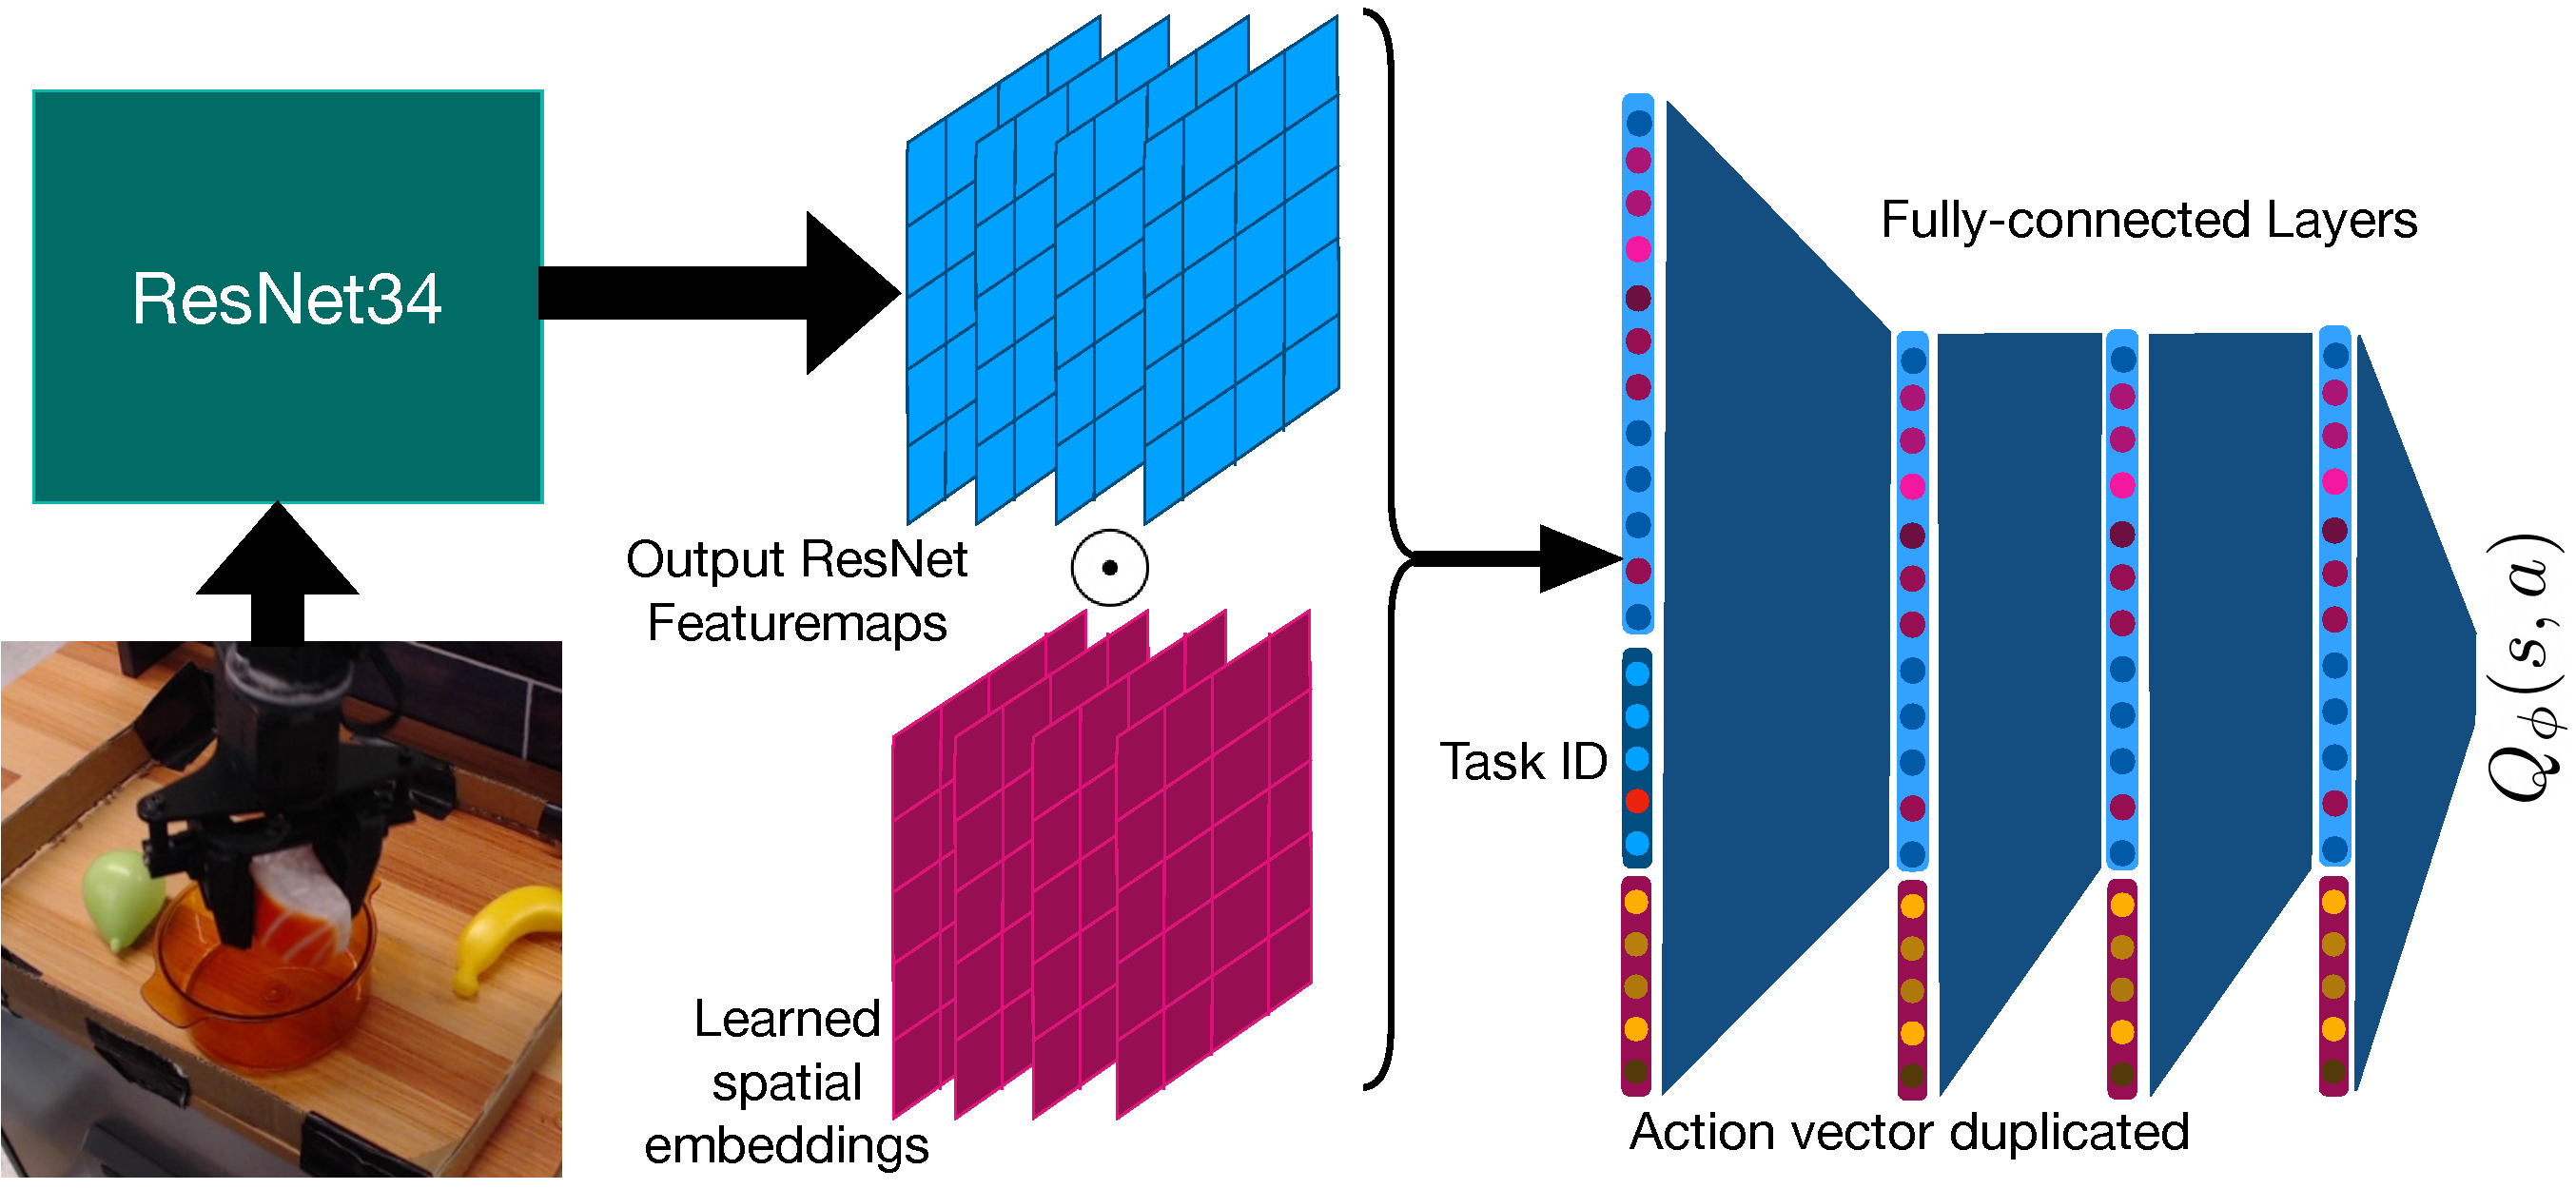
\includegraphics[width=0.85\linewidth]{chapters/ptr/architecture.pdf}
  \caption{\footnotesize{\textbf{Q-function architecture for \ptrmethodname.} The encoder is a ResNet34 with group normalization along with learned spatial embeddings (left). The decoder (right) is a MLP with the action vector duplicated and passed in at each layer. A one-hot task identifier is also passed into the input of the decoder.}}
  \vspace{-0.1cm}
  \label{fig:arch}
\end{figure}

~

\niparagraph{\large{\textbf{Policy and Q-function architectures}}}
~

Perhaps the most crucial design decision for our approach is the neural network architecture for representing $\pi^\text{off}$ and $Q^\text{off}$. Since we wish to fine-tune the policy for different tasks, we must use high-capacity neural network models for representing the policy and the Q-function. We experimented with a variety of standard (high-capacity) architectures for vision-based robotic RL. This includes standard convolutional architectures~\citep{singh2020cog} and IMPALA architectures~\citep{espeholt2018impala}. However, we observed in Figure~\ref{fig:scaling_ptr} that these {standard models were unable to effectively handle the diversity of the pre-training data} and performed poorly.
Then, we attempted to utilize standard ResNets~\citep{resnet} (ResNet-18, Resnet-34, and their adaptations to imitation problems from \citet{ebert2021bridge}) to represent $Q_\phi$, but faced divergence challenges similar to prior efforts that use batch normalization~\citep{bjorck2021towards,2019arXiv190205605B} in the Q-network. Batch normalization layers are known to be hard to train with TD-learning~\citep{2019arXiv190205605B} and, therefore, by replacing batch normalization layers with \textcolor{brown}{\textbf{group normalization}} layers~\citep{wu2018group}, we were able to address such divergence issues.
See Appendix~\ref{app:design} for quantitative studies comparing these choices. Unlike prior work~\citep{lee2022multi}, we observed that with group normalization, we attain favorable scaling properties of \ptrmethodname: the more the parameters, the better the performance as shown in Figure~\ref{fig:scaling_ptr}.
We also observed that choosing an appropriate method for converting the three-dimensional feature-map tensor produced by the ResNet into a one-dimensional embedding plays a crucial role for learning accurate Q-functions and obtaining functioning policies. Unlike standard ResNet architectures for supervised learning, simply utilizing global average pooling (as used in many classification architectures) performs poorly. Instead we point-wise multiply the learned feature-map with a 3-dimensional parameter tensor before computing sums over the spatial dimensions which allows the network to explicitly encode spatial information. {We refer to this technique as ``\textcolor{brown}{\textbf{learned spatial embeddings}}''}. An illustration of this architecture is provided in \autoref{fig:arch}. As detailed in Appendix~\ref{app:design}, Table~\ref{tab:spatial}, {we find that utilizing this technique leads to improved performance}.

Next, we found that a Q-function $Q_\phi(\bs, \mathbf{a})$ obtained by running na\"ive multi-task CQL on the demonstration data tends to not use the action input $\mathbf{a}$ effectively, due to strong correlations between $\bs$ and $\mathbf{a}$ in the data, which is almost always the case for narrow, human demonstrations. As a result, policy improvement against such a Q-function overfits to these correlations, producing poor policies. To resolve this issue, we modified the architecture of Q-network to \textcolor{brown}{\textbf{pass the action \textbf{\textit{$\mathbf{a}$}} as input to every fully-connected layer}} which, as shown in \autoref{fig:arch} and {Appendix~\ref{app:design}}, {Table~\ref{tab:action_sep}}), greatly alleviates the issue {and significantly improves over na\"ive CQL}. 

~

\niparagraph{\large{\textbf{Cross-validation during offline fine-tuning}}} 


As we wish to learn task-specific policies that do not overfit to small amounts of data, we must apply the right number of gradient steps during fine-tuning: too few gradient steps will produce policies that do not succeed at the target tasks, while too many gradient steps will give policies that have likely lose the generalization ability of the pre-trained policy. {To handle this trade-off, we adopt the following heuristic as a loose guideline:} we run fine-tuning for many iterations while also plotting the learned Q-values over a held-out dataset of trajectories from the target task as seen in Figure~\ref{fig:moreexreb}. Then for evaluation, we pick the checkpoints that presented a Q-function with the Q-values appearing closest to having a monotonically increasing trend in a trajectory. This is a \emph{relative} guideline and must be performed within the checkpoints observed within a run. The reason for this heuristic choice is that a valid Q-function must be a valid estimator for discounted return, and hence, it must increase over time-steps of a trajectory for a given task.  Of course, this heuristic does not hold for arbitrary sub-optimal offline data, but all of our data comes from human-collected demonstrations. In principle, this heuristic can be wrapped into a metric quantifying degree of monotonicity of the Q-value curve in Figure~\ref{fig:moreexreb}, but in our experiments, we felt this was not necessary: as we show below, we were able to narrow down the checkpoints to essentially one or at most, two checkpoints by just visual inspection. Of course, designing an accurate metric would be helpful for future work. We present two worked-out examples of our checkpoint selection strategy for two tasks from Scenario 1 and Scenario 3 in Figure~\ref{fig:moreexreb}. Observe that checkpoints early in training exhibit Q-values that fluctuate arbitrarily at the beginning of training, which is clearly non-monotonic. This is because of the lack of sufficient gradient steps for fine-tuning the target task. Once sufficient gradient steps are performed, the Q-values visibly improve on the monotonicity property. Training further leads to much flatter Q-values, that are visibly less monotonic. 


\begin{figure}[h]
\centering
  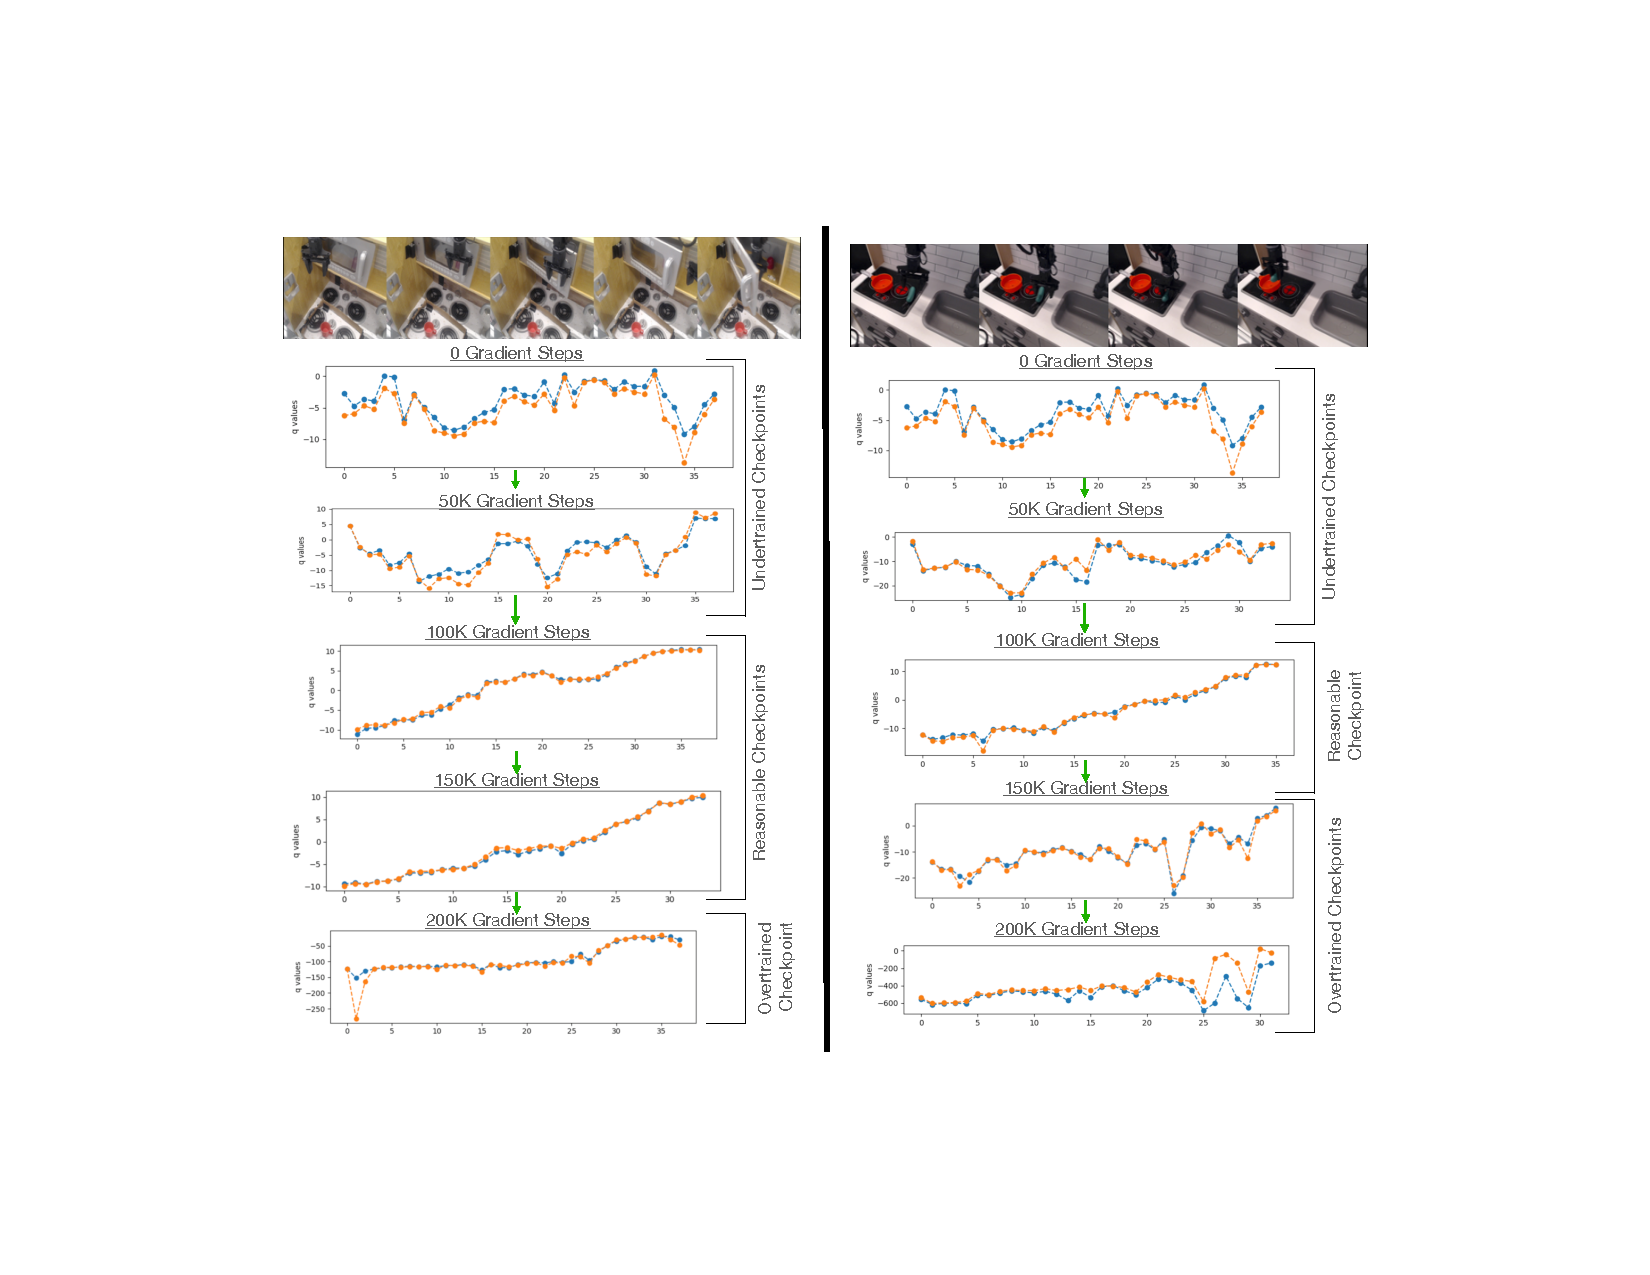
\includegraphics[width=0.6\linewidth]{chapters/ptr/Fig_rebuttal.pdf}
  \vspace{-0.1cm}
  \caption{\footnotesize \textbf{Evolution of Q-values on the target task over the process of fine-tuning with \ptrmethodname.} Observe that while the learned Q-values on \emph{held-out} trajectories from the dataset just at the beginning of Phase 2 (fine-tuning) do not exhibit a roughly increasing trend, we choose to evaluate those checkpoints of \ptrmethodname that exhibit a visible more increasing trend in the Q-values despite having access to only 10 demonstrations for these target tasks.}
  \label{fig:moreexreb}
  \vspace{-0.1cm}
\end{figure}

To validate our checkpoint selection mechanism, in Figure~\ref{fig:validation_door} we present a film-strip of a sample evaluation of a good and a poor checkpoint as identified by the cross-validation strategy mentioned above. We observe that the checkpoint with more flat Q-values fails to solve the door opening task, whereas the one with a visibly increasing Q-value trend solves the task.

\begin{figure}[h]
\centering
\vspace{-0.2cm}
  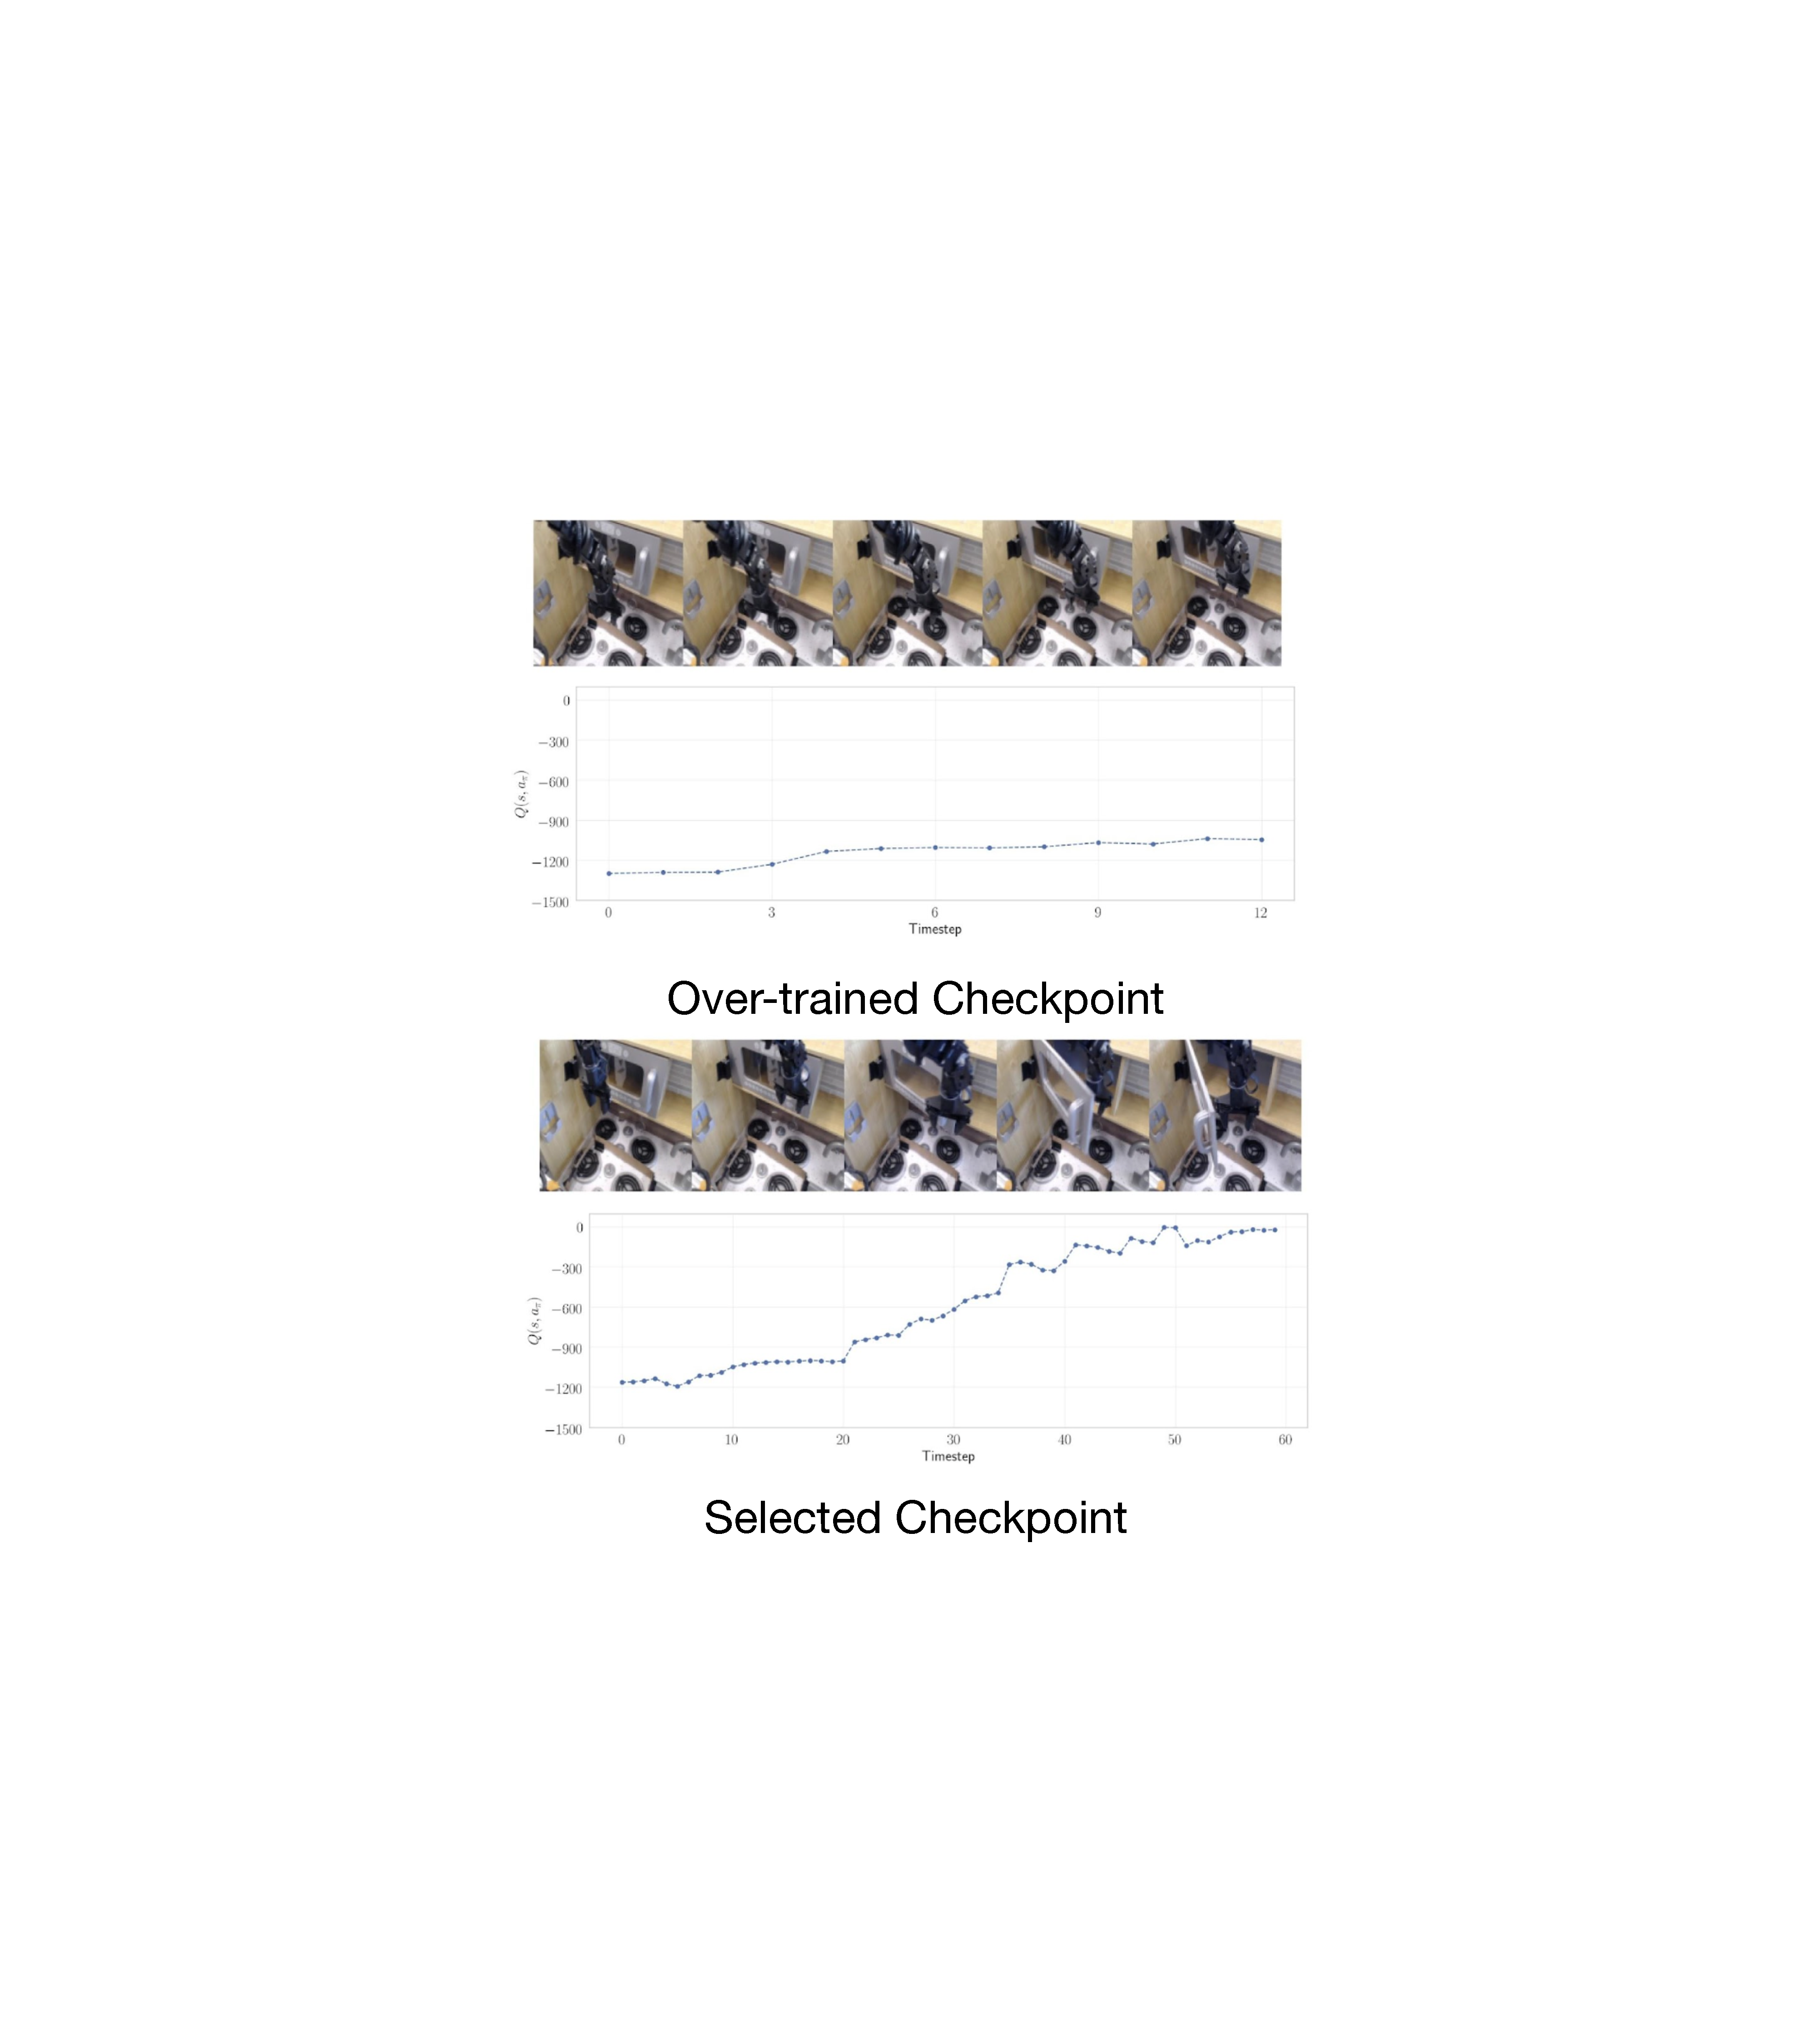
\includegraphics[width=0.6\linewidth]{chapters/ptr/fig_chkpt.pdf}
  \vspace{-0.1cm}
  \caption{\footnotesize \textbf{Performance evaluation of a selected and over-trained checkpoint of \ptrmethodname.} We validate our checkpoint selection mechanism on the door opening task. An over-trained checkpoint with nearly flat Q-values fails to solve the task, whereas a checkpoint with visibly increasing Q-values solves the task.}
  \label{fig:validation_door}
  \vspace{-0.2cm}
\end{figure}

~

\niparagraph{\large{\textbf{Reward specification}}} 


In this paper, we aim to pre-train on existing robotic datasets, such as the Bridge Dataset~\citep{ebert2021bridge}, which consists of human-teleoperated demonstration data. Although the demonstrations are all successful, they are not annotated with any reward function. Perhaps an obvious choice is to label the last transition of each trajectory as success, and give it a +1 binary reward. However, in several of the datasets we use, there can be a 0.5-1.0 second lag between task completion and when the episode is terminated by the data collection. To ensure that a successful transition is not incorrectly labeled as $0$, we utilized the practical heuristic of annotating the last $n=3$ transitions of every trajectory with a reward of $+1$ and and annotated other states with a $0$ reward. We show in Appendix~\ref{app:exp_results} that this provided the best results. 
In principle, more complicated methods of reward labeling~\citep{eysenbach2021replacing} could be used. However, we found the presented rule to be simple and yet effective to learn good policies.



\begin{figure*}
\centering
  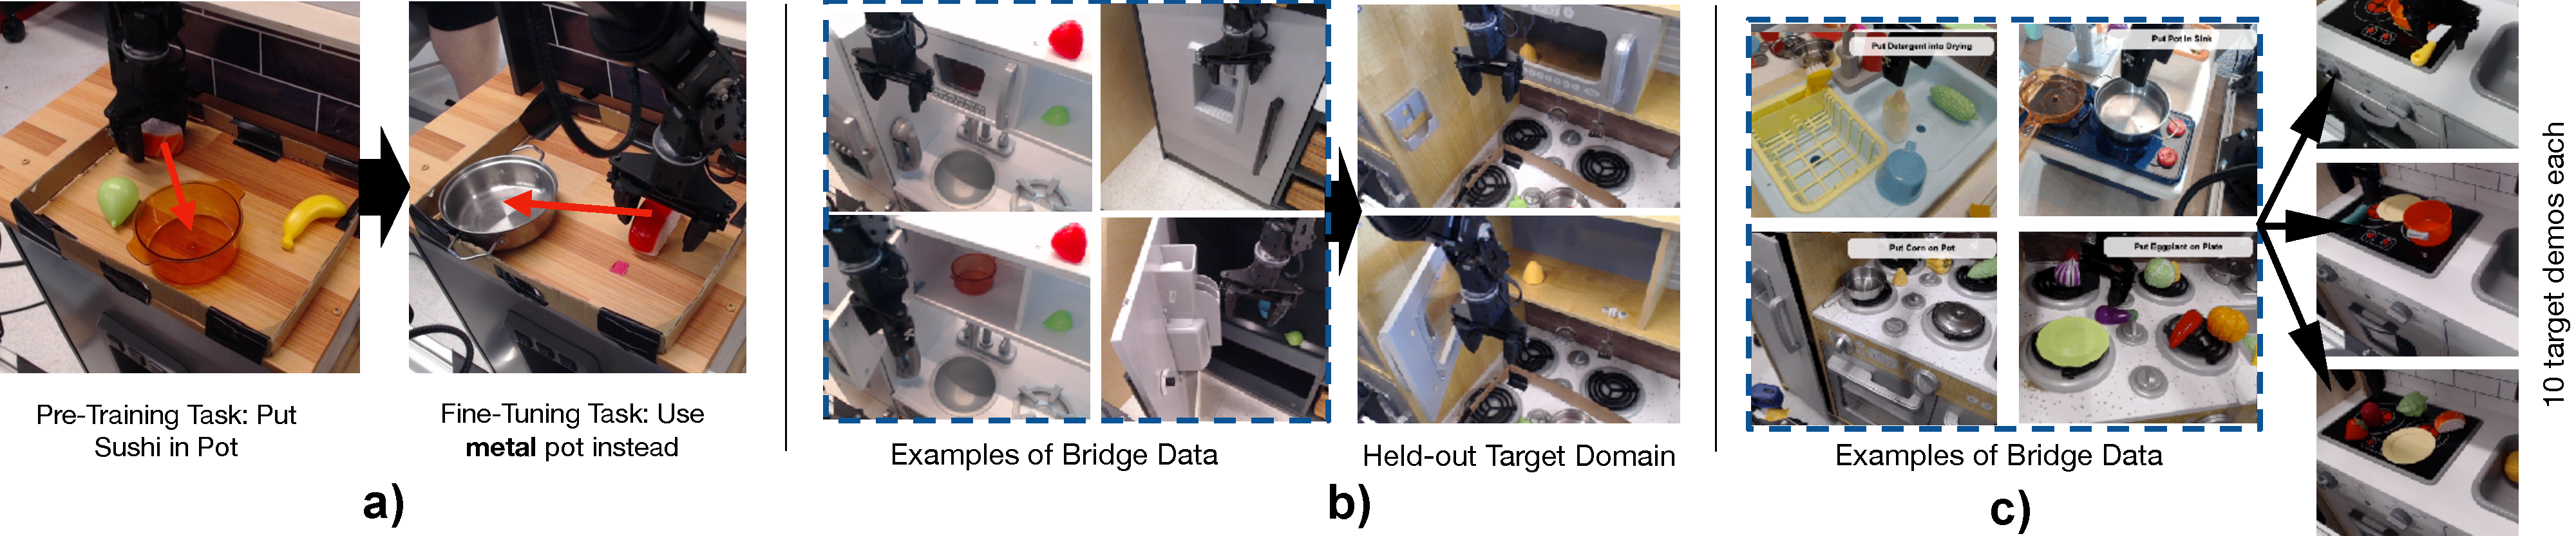
\includegraphics[width=0.8\linewidth]{chapters/ptr/scenarios_overview.pdf}
  % \vspace{-0.45cm}
  \caption{\footnotesize{\textbf{Illustrations of the three real-world experimental setups we evaluate \ptrmethodname on:} \textbf{(a)} the ``put sushi in a metallic pot'' task which requires retargeting, \textbf{(b)} the task of opening an unseen door, and \textbf{(c)} fine-tuning on several novel target tasks in a held out toykitchen environment.}}
  \vspace{-0.6cm}
  \label{fig:experiments}
\end{figure*}


\vspace{0.1cm}
\section{Experimental Evaluation of \ptrmethodname and Takeaways for Robotic RL}
\label{sec:result}
\vspace{0.1cm}
The goal of our experiments is to validate if \ptrmethodname\ can learn effective policies from only a handful of user-provided demonstrations for a target task, by effectively utilizing previously-collected robotic datasets for pre-training. We also aim to understand whether the design decisions introduced in Section~\ref{sec:design_choices} are crucial for attaining good robotic manipulation performance. To this end, we evaluate \ptrmethodname\ in a variety of robotic manipulation settings, and compare it to state of the art methods, which either do not use offline RL or do not learn end-to-end by employing some form of visual representation learning. We evaluate in three scenarios: \textbf{(a)} when the target task requires retargeting the behavior of an existing skill, in this case changing the type of object types it interacts with, \textbf{(b)} when the target task requires performing a previously observed task but this time in a previously unseen domain, and \textbf{(c)} when the target task requires learning a new skill in a new domain, by using the target demonstrations. We also perform a diagnostic study in simulation in Appendix~\ref{app:sim_diagnostic} (Table~\ref{tab:sim_complete}). 


\vspace{0.1cm}
\subsection{Setup and Comparisons}
\vspace{0.1cm}

\textbf{Real-world experimental setup.} We directly utilize the publicly available \emph{Bridge Dataset}
\cite{ebert2021bridge} for pre-training, as it provides a large number of robot demonstrations for a diverse set of tasks in multiple domains, i.e., multiple different toy kitchens. We use the same WidowX250 robot platform for our evaluations. The bridge dataset contains distinct tasks, each differing in terms of the objects that the robot interacts with and the domain the task is situated in. We assign a different task identifier to each task in the dataset for pre-training. We also evaluate on an additional door-opening task not present in the Bridge Dataset, where we collected demonstrations for opening and closing a variety of doors, and test our system on new, unseen doors. {More details are in Appendix~\ref{app:exp_setup}.} 



\textbf{Comparisons.} Since the datasets we use (both the pre-training bridge dataset from \citep{ebert2021bridge} and the newly collected door opening data) consist of human demonstrations, as indicated by prior work~\citep{mandlekar2021what}, the strongest prior method in this setting is behavioral cloning (BC), which attempts to simply imitate the action of the demonstrator based on the current state. We incorporate BC in a pipeline similar to \ptrmethodname, denoted as \textbf{BC (finetune)}, where we first run BC on the pre-training dataset, and then finetune it using the demonstrations on the target task using the same batch mixing as in \ptrmethodname. 
To ensure that our BC baselines are well-tuned, we utilize standard practices of cross-validation via a held-out validation set to tune hyperparameters and make early stopping decisions are we elaborate on in {Appendix~\ref{app:hyperparams}}.
Next, to assess the importance of performing pre-training \emph{followed} by fine-tuning, we compare \ptrmethodname to \textbf{(i)} jointly training on the pre-training and fine-tuning data with CQL, which is equivalent to the COG approach of \citet{singh2020cog},
\textbf{(ii)} multi-task offline CQL (\textbf{CQL (zero-shot)}) that does not use the target demonstrations at all, and \textbf{(iii)} utilizing CQL to train on target demonstrations alone from scratch, with no pre-training data included (\textbf{CQL (target data only)}).
We also make the analogous comparison for BC, jointly training BC on the pre-training and target task data from scratch (\textbf{BC (joint)}) which is equivalent to \citep{ebert2021bridge}. For fairness of comparison, BC, CQL, and \ptrmethodname (both for zero-shot, joint-training and fine-tuning) use the \emph{same} exact architecture, including our learned-spatial embedding described in Section~\ref{sec:design_choices}.


\vspace{0.1cm}
\subsection{Experimental Results}
\vspace{0.1cm}

\begin{table}[h]
% \small{
% \vspace{-0.5cm}
\centering
% \vspace*{0.1cm}
\resizebox{0.5\linewidth}{!}{\begin{tabular}{l|r}
\toprule
\textbf{Method} & \textbf{Success rate}\\ \midrule
BC (zero-shot) & 0/30 \\
BC (finetune) & 0/30  \\ 
CQL (zero-shot) & 2/30 \\
\midrule
\textbf{\ptrmethodname (Ours)} & \textbf{14/30} \\ 
\bottomrule
\end{tabular}
}
\vspace{-0.2cm}
\caption{\footnotesize{\textbf{Performance of \ptrmethodname for ``put sushi in metallic pot'' in Scenario 1.} \ptrmethodname substantially outperforms BC (finetune), even though it is provided access to only demonstration data. We also show some examples comparing some trajectories of BC and \ptrmethodname in Appendix ~\ref{app:exp_results}.}}
\label{tab:retarget}
% }
\vspace{-0.2cm}
\end{table}

\begin{table*}[h]
% \small{
% \vspace{-0.5cm}
\centering
% \vspace*{0.1cm}
\resizebox{0.65\linewidth}{!}{
\begin{tabular}{c|c||c|c|c|c|c|c|c}
    \toprule
    & & & \multicolumn{2}{c|}{\textbf{zero-shot}} &  \multicolumn{2}{c|}{\textbf{Joint Training}} & \multicolumn{2}{c}{\textbf{Target data only}} \\
    \midrule
      {\textbf{Task}} & \textbf{\ptrmethodname (Ours)} & \textbf{BC (fine.)}   & \textbf{CQL} & \textbf{BC} & \textbf{COG} & \textbf{BC}& \textbf{CQL} & \textbf{BC} \\
    \midrule
   Open Door & \textbf{12/20} & 10/20 & 0/20 & 0/20 & 5/20  & 7/20 &  4/20  & 7/20  \\
    \bottomrule
    \end{tabular}
}
\caption{\footnotesize{{\textbf{Successes vs. total trials for opening a new target door in Scenario 2}}. \ptrmethodname outperforms both BC (finetune) and BC (joint) given access to the same data. Note that joint training is worse than finetuning from the pre-trained initialization.}}
\label{tab:adapting}
% }
\vspace{-0.5cm}
\end{table*}

\textbf{Scenario 1: Re-targeting skills for existing tasks to handle new objects.} We utilized the subset of the bridge data with pick-and-place tasks in one toy kitchen for pre-training, and selected the ``put sushi in pot'' task as our target task. This task is depicted in the bridge dataset, but only using an orange transparent pot (see \autoref{fig:experiments} (a)). In order to construct a scenario where the offline policy at the end of pre-training must be re-targeted to act on a different object, we collected only \emph{ten} demonstrations that place the sushi in a metallic pot and used these demonstrations for fine-tuning.
This scenario is challenging since the metallic pot differs significantly from the orange transparent pot visually. 
By pre-training on all pick-and-place tasks in this domain (32 tasks) and fine-tuning on this data and 10 demonstrations, \ptrmethodname\ is able to obtain a policy that is re-targeted towards the metal pot. On the other hand, the policy learned by BC confuses arbitrary patches on the tabletop with the pot. Quantitatively, observe in \autoref{tab:retarget} that \ptrmethodname is able to complete the task with reasonable accuracy across a set of easy and hard initial positions, whereas zero-shot and fine-tuned BC are completely unable to solve the task. The fact that zero-shot CQL has difficulty solving the task indicates that target demonstrations are necessary, and \ptrmethodname is able to attain successful behavior with just ten demonstrations.

\textbf{Scenario 2: Generalizing to previously unseen domains.} Next, we study whether \ptrmethodname can adapt behaviors seen in the pre-training data to new domains. We study a door opening task, which requires significantly more complex maneuvers and precise control compared to the pick-and-place tasks from above (as seen in the video present in the supplementary material and our \hyperlink{https://sites.google.com/view/ptr-rss}{anonymous website}).
The doors in the pre-training data exhibit different sizes, shapes, handle types and visual appearances, and the target door (shown in \autoref{fig:experiments}(b)) we wish to open and the corresponding toy kitchen domain are never seen previously in the pre-training data. Concretely, for pre-training, we used a dataset of 800 door-opening demonstrations on 12 different doors in 4 different toy kitchen domains, and we utilize 15 demonstrations on a held-out door for fine-tuning. \autoref{tab:adapting} shows that \ptrmethodname improves over both BC baselines and joint training with CQL (or COG). Due to the limited target data and the associated task complexity, in order to succeed, an method must effectively leverage the pre-training data to learn a general policy that attempts to solve the task, and then specialize it to the target door.

Interestingly, \autoref{tab:adapting} shows that while jointly training on the pre-training and fine-tuning data (or COG~\citep{singh2020cog}) by itself does not outperform BC (joint), the pre-training and fine-tuning approach in \ptrmethodname{} leads to significantly better performance, improving over the best BC approach. Since CQL (joint) is equivalent to \ptrmethodname{}, but with no Phase 1, this large performance gap indicates the efficacy of offline RL methods trained on large diverse datasets at providing good initializations for learning new downstream tasks. We believe that this finding may be of independent interest to robotic offline RL practitioners: when utilizing multi-task offline RL, it might be better first to run multi-task pre-training followed by fine-tuning, as opposed to jointly training from scratch.


\begin{table*}
    \centering
    % \vspace{-0.15cm}
    \resizebox{0.9\linewidth}{!}{\begin{tabular}{c||c||c|cc|cc|cc|c}
    \toprule
    & &  \multicolumn{3}{c|}{\textbf{BC finetuning}} & \multicolumn{2}{c|}{\textbf{Joint training}} &  \multicolumn{2}{c|}{\textbf{Target data only}} &  {\textbf{Meta-learning}} \\
    \midrule
      {\textbf{Task}} & \textbf{\ptrmethodname (Ours)} & \textbf{BC (fine.)} & \textbf{Autoreg. BC}& \textbf{BeT} &\textbf{{COG}} & \textbf{{BC}} & \textbf{CQL} & \textbf{BC} & {\textbf{MACAW}} \\
    \midrule
    Take croissant from metal bowl & \textbf{7/10} & 3/10 & 5/10 & 1/10 & 4/10 & 4/10 & 0/10 & 1/10  & 0/10 \\
    Put sweet potato on plate & \textbf{7/20} & 1/20 & 1/20 & 0/20 & 0/20 & 0/20 & 0/20 & 0/20 & 0/20 \\
    Place knife in pot & \textbf{4/10} & 2/10 & 2/10 & 0/10 & 1/10 & 3/10 & 3/10 & 0/10 & 0/10 \\
    Put cucumber in pot & \textbf{5/10} & 0/10 & 1/10 & 0/10 & 2/10 & 1/10 & 0/10 & 0/10 & 0/10 \\
    \bottomrule
    \end{tabular}}
    % \vspace{-0.3cm}
    \caption{\footnotesize{\textbf{Performance of \ptrmethodname and other baseline methods for new tasks in Scenario 3.} Note that \ptrmethodname outperforms all other baselines including BC (finetune), BC with more expressive policy classes (BeT~\citep{shafiullah2022behavior}, Auto-regressive), offline RL with no pre-training (``Target data only'') and joint training~\citep{singh2020cog,ebert2021bridge}. PTR also outperforms few-shot gradient-based meta learning methods such as MACAW~\citep{mitchell2021offline}, which fail to attain non-zero performance.}}
    \label{tab:scenario4}
    % \vspace{-0.3cm}
\end{table*}


\textbf{Scenario 3: Learning to solve new tasks in new domains.} 
Finally, we evaluate the efficacy of \ptrmethodname in learning to solve a new task in a new domain. 
This scenario presents a generalization requirement that is significantly more challenging than the previously studied scenarios, since both the task and the domain are never seen before. This task is represented via a new task identifier, and pre-training receives no data for this task identifier, or even any data from the kitchen where this task is situated. We pre-train on all 80 pick-and-place style tasks from the bridge dataset, while holding out any data from the new task kitchen, and then fine-tune on 10 demonstrations for 4 target tasks independently in this new kitchen, as shown in Table~\ref{tab:scenario4}. 
Methods that utilize more expressive policy architectures (an auto-regressive policy or behavior transformers (BeT)~\citep{shafiullah2022behavior}) do not lead to improved performance compared to the standard BC (finetune) approach, and we find that PTR outperforms these approaches. Please find more details on the implementation of auto-regressive BC and BeT in Section \ref{app:hyperparams}. This might appear surprising, and perhaps just a hyper-parameter tuning artifact at first, but we present additional qualitative and quantitative analysis aiming at understanding the reasons behind why our offline RL-based PTR approach works better in Section~\ref{sec:rl_vs_bc}. We also compare to MACAW~\citep{mitchell2021offline}, an offline meta-RL method that utilizes advantage-weighted regression~\citep{peng2019awr} for gradient-based few-shot adaptation, and find that this approach is unable to learn policies that succeed. We discuss the hyperparameter configurations that we tried for this approach in Appendix \ref{app:scenario4}. Finally, observe in Table~\ref{tab:scenario4} that joint training with CQL or BC, or just using target data, without any pre-training for CQL or BC, all perform significantly worse than PTR.

\begin{table}
    \centering
    % \vspace{-0.15cm}
    \resizebox{0.8\linewidth}{!}{\begin{tabular}{c||c||cc}
    \toprule
    & &  \multicolumn{2}{c}{\textbf{Pre-train. rep. + BC finetune}} \\
    \midrule
      {\textbf{Task}} & \textbf{\ptrmethodname (Ours)} & \textbf{R3M} & \textbf{MAE} \\
    \midrule
    Take croissant from bowl & \textbf{7/10} & 1/10 & 3/10 \\
    Put sweet potato on plate & \textbf{7/20} & 0/20 & 1/20  \\
    Place knife in pot & \textbf{4/10}  & 0/10 & 0/10  \\
    Put cucumber in pot & \textbf{5/10}  & 0/10 & 0/10 \\
    \bottomrule
    \end{tabular}}
    % \vspace{-0.3cm}
    \caption{\footnotesize{\textbf{Performance of \ptrmethodname and other pre-training methods (R3M and MAE).} While both R3M~\citep{nair2022r3m} and MAE~\citep{xiao2022masked} help improve performance over na\"ively applying BC on the target data, \ptrmethodname outperforms both.}}
    \label{tab:rep_learning_comparison}
    \vspace{-0.6cm}
\end{table}

\vspace{0.05cm}
\subsection{Comparison to non-RL Visual Pre-Training Methods}
\vspace{0.05cm}

We also compare PTR to approaches that utilize the diverse bridge dataset or Internet-scale data
for task-agnostic visual representation learning, followed by down-stream behavioral cloning only on the target fine-tuning task which utilizes the representation learned during pre-training. In particular, we compare to two approaches: R3M~\citep{nair2022r3m}, which utilizes the Ego4D dataset of human videos to obtain a representation, and MVP~\citep{radosavovic2022real,xiao2022masked}, which trains a masked auto-encoder~\citep{he2111masked} on the Bridge Dataset and utilizes the learned latent space as the representation of the new image. Observe in Table~\ref{tab:rep_learning_comparison} that, while utilizing R3M or MAE does improve over running BC on the target data alone (compare R3M and MAE in Table~\ref{tab:rep_learning_comparison} to BC on target data only in Table~\ref{tab:scenario4}), the pre-training scheme from PTR outperforms both of these prior pre-training approaches, indicating the efficacy of offline RL pre-training on diverse robot data in recovering useful representations for downstream policy learning.




\vspace{0.1cm}
\subsection{Understanding the Benefits of PTR over BC}
\label{sec:rl_vs_bc}
\vspace{0.1cm}


One natural question to ask given the results in this paper is: why does utilizing an offline RL method for pre-training and fine-tuning as in \ptrmethodname outperform BC-based methods even though the dataset is quite ``BC-friendly'', consisting of only demonstrations? The answer to this question is not obvious, especially since joint training with BC still outperforms jointly training with CQL on both pre-training and target demonstration data (COG) in our results in Table~\ref{tab:scenario4}.  

To understand the reason behind improvements from RL, we perform a qualitative evaluation of the policies learned by PTR and BC (finetune) on two tasks: take croissant from metal bowl and put cucumber in bowl in Figure~\ref{fig:dumb_behavior}. We find that the failure mode of BC policies can be primarily explained as a lack of precision in locating the object, or a prematurely-executed grasping action. This is especially prevalent in settings where the object of interest is farther away from the robot gripper at the initial state, and hints at the inability of BC to prioritize learning the critical decisions (e.g., precisely moving over the object before the grasping action) over non-critical ones (e.g., the action to take to reach nearby the object from farther away). On the other hand, RL can learn to make such critical decisions correctly as shown in Figure~\ref{fig:dumb_behavior}. We present additional rollouts in Appendix~\ref{app:exp_setup}.

\begin{figure}[h]
\centering
\vspace{-0.4cm}
  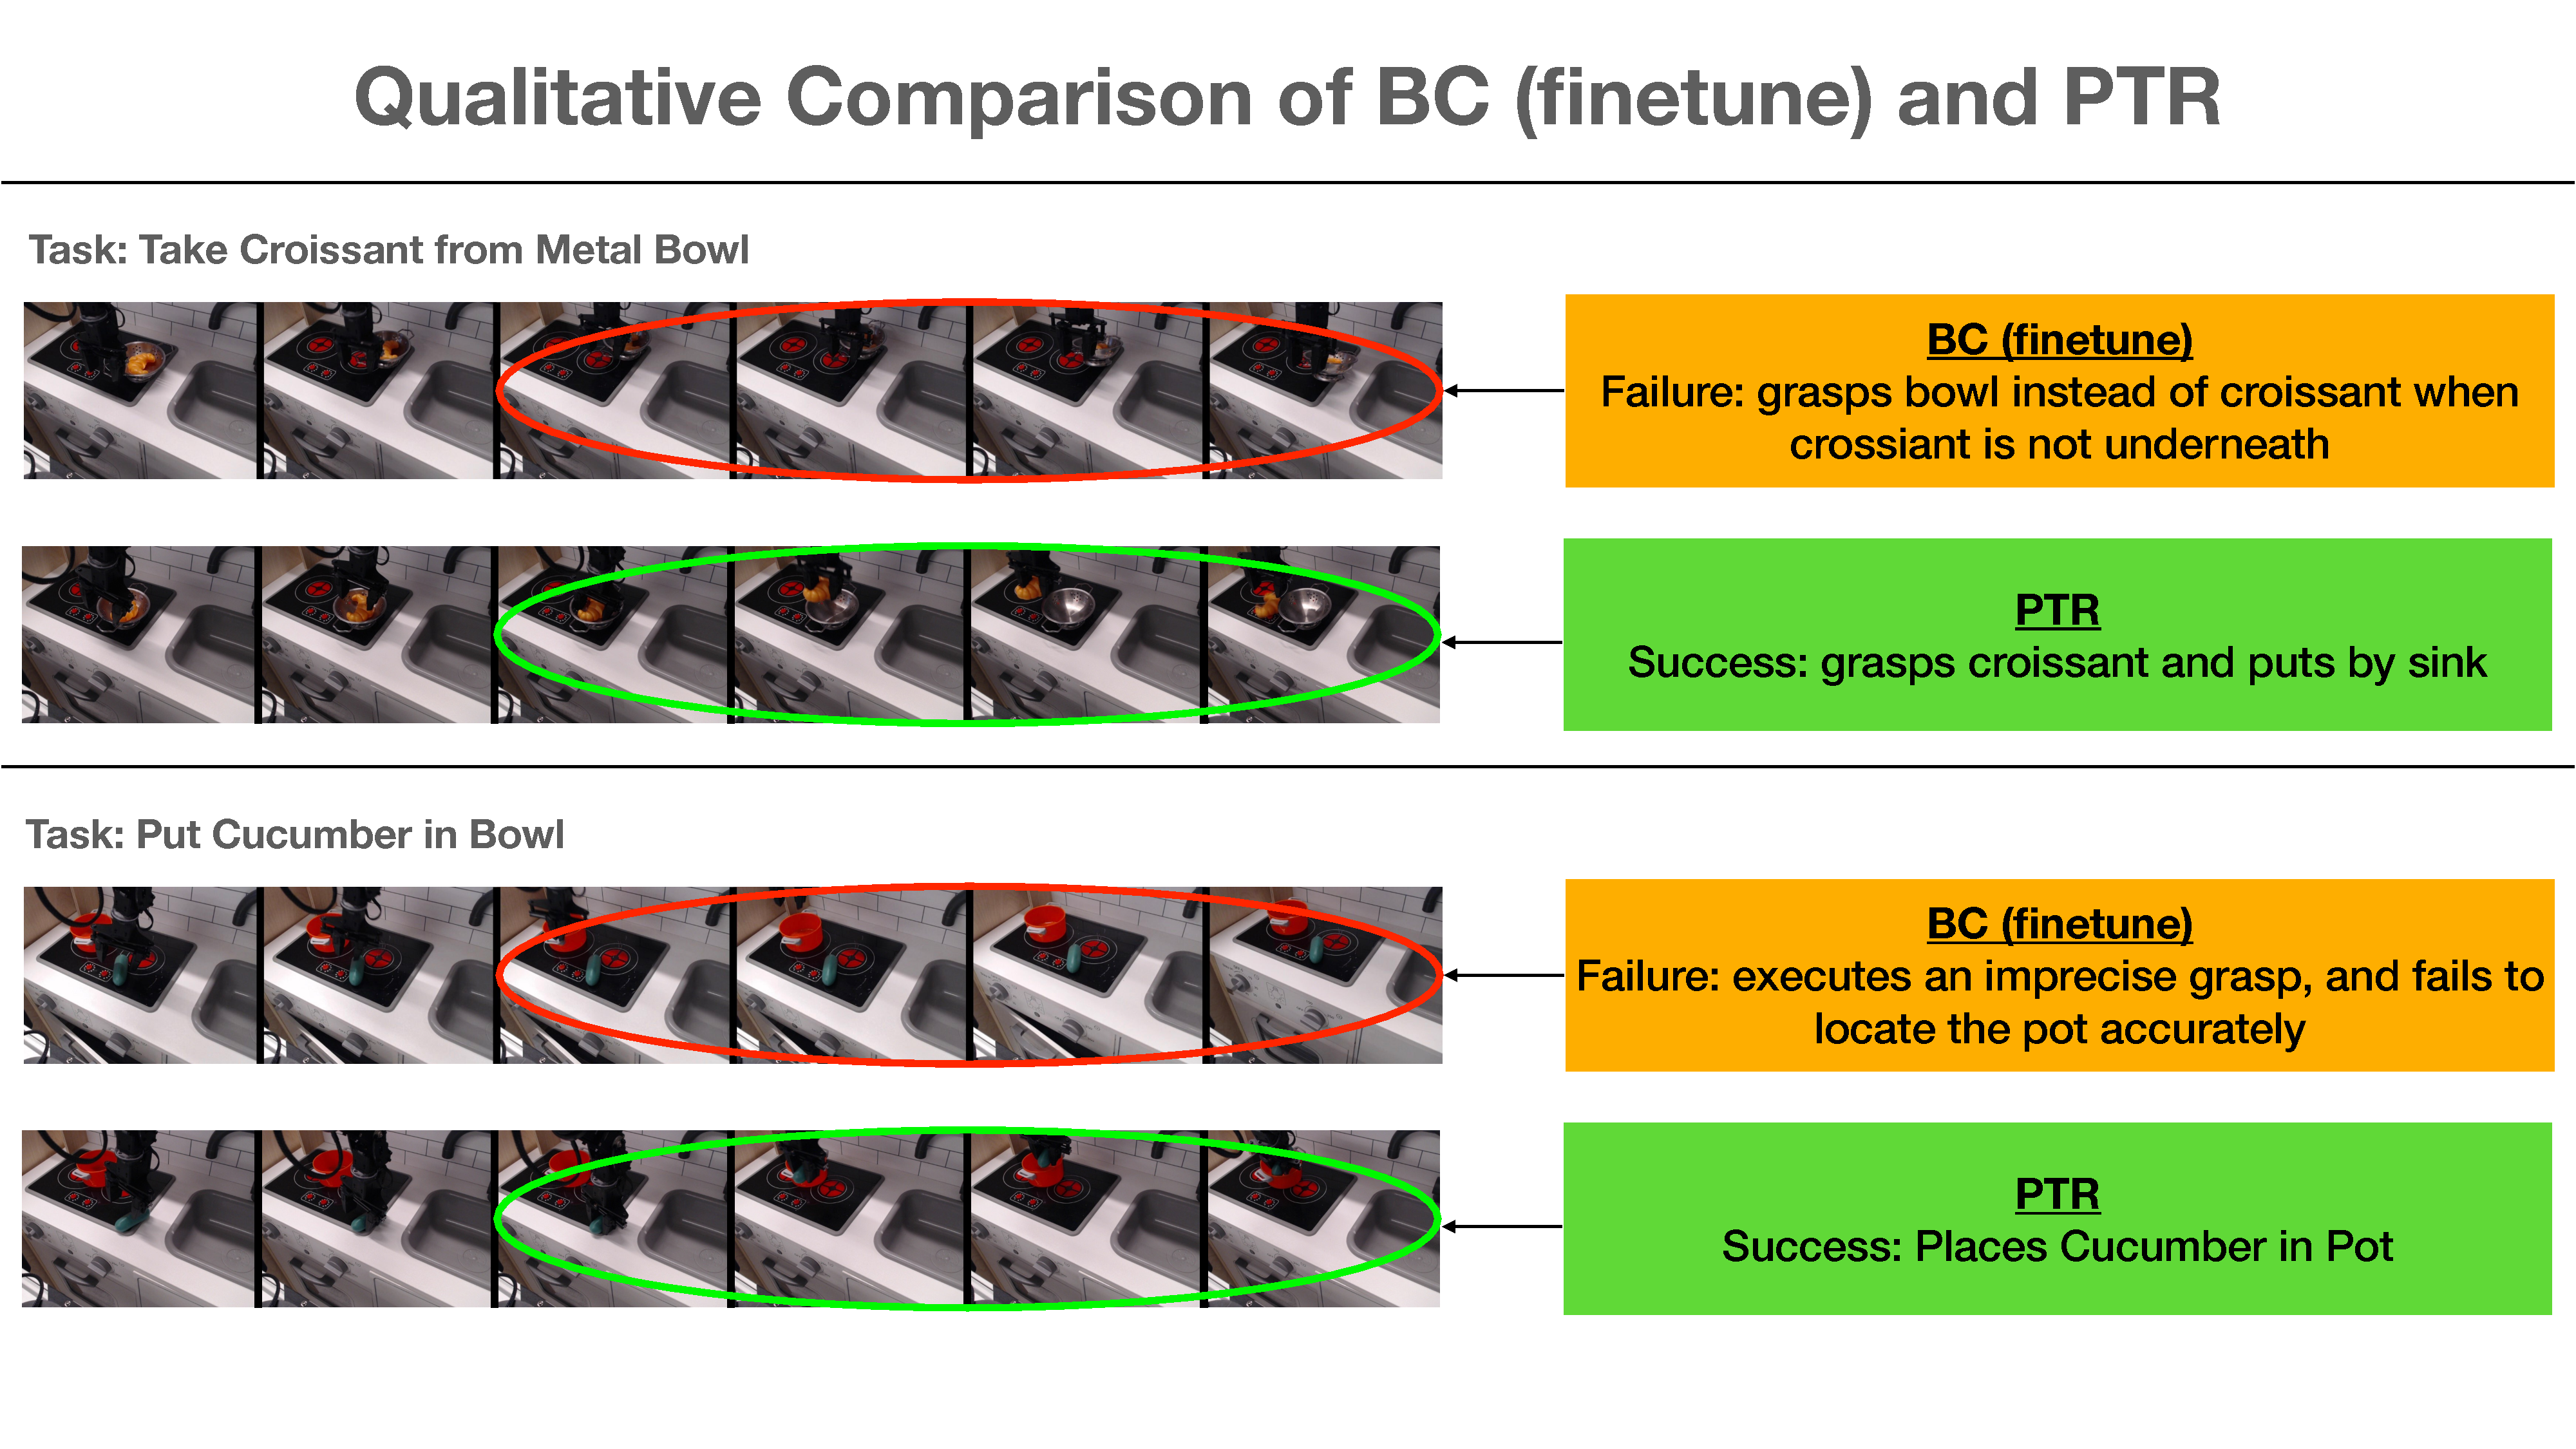
\includegraphics[width=0.8\linewidth]{chapters/ptr/Comparison.pdf}
  \vspace{-0.3cm}
  \caption{\footnotesize \textbf{Qualitative successes of \ptrmethodname visualized alongside failures of BC (fine-tune).} As an example, observe that while \ptrmethodname is accurately able to reach to the croissant and grasp it to solve the task, BC (finetune) is imprecise and grasps the bowl instead of the croissant resulting in failure.}
  \label{fig:dumb_behavior}
  \vspace{-0.3cm}
\end{figure}


\begin{table}[h]
% \small{
\centering
% \vspace{0.1cm}
\resizebox{0.75\linewidth}{!}{\begin{tabular}{c|r|r||r}
\toprule
\textbf{Task} & \textbf{BC (finetune)} & \textbf{\ptrmethodname} &\textbf{AW-BC (finetune)}  \\ \midrule
Cucumber &  0/10 & 5/10 &  {5/10} \\
Croissant & 3/10 &  7/10  & {6/10} \\
\bottomrule
\end{tabular}}
% \vspace{-0.3cm}
\caption{\footnotesize{\textbf{Performance of advantage-weighted BC} on two tasks from Table~\ref{tab:scenario4}. Observe that weighting the BC objective using advantage estimates from the Q-function learned by \ptrmethodname leads to much better performance than standard BC (finetune), almost recovering PTR performance. This test indicates that the Q-function in \ptrmethodname allows us to be accurate on the more critical decisions, thereby preventing the failures of BC.}}
\vspace{-0.3cm}
\label{tab:aw_bc}
\end{table}

Next, to verify if the performance benefits can be explained by the ability of Q-learning to prioritize critical decisions, we run a form of weighted behavioral cloning, where the weights $w_\phi(\bs, \ba)$ are derived from the \emph{advantage estimates computed using a frozen Q-function learned by PTR} after fine-tuning:
\begin{align*}
    w_\phi(\bs, \ba)  \propto \exp(Q_\phi(\bs, \ba) - \max_{\ba'} Q_\phi(\bs, \ba')).
\end{align*}
Note that this is not the same as standard advantage-weighted regression~\citep{peng2019awr}, which uses Monte-Carlo return estimates for computing advantage weights instead of using advantages computed under a Q-function trained via PTR or CQL. As shown in Table~\ref{tab:aw_bc}, we find that this advantage-weighted BC (AW-BC) approach performs significantly better than BC (finetune) method and comparably to PTR, for two tasks (croissant and cucumber from Table~\ref{tab:scenario4}. Since AW-BC is essentially the same as BC, just with a modified weight to indicate the importance of any transition, this performance improvement clearly indicates the benefits of learning value functions via PTR in a pre-training then fine-tuning setting, even when we only have demonstration data.  Note that since AW-BC uses the PTR-derived weights after fine-tuning, it cannot serve as an independent method, but rather amounts to another way to use the PTR value function.


% \vspace{-0.06cm}
\subsection{Effective Use of High-Capacity Neural Networks}
\vspace{0.1cm}

\begin{figure}
\centering
\vspace{-0.7cm}
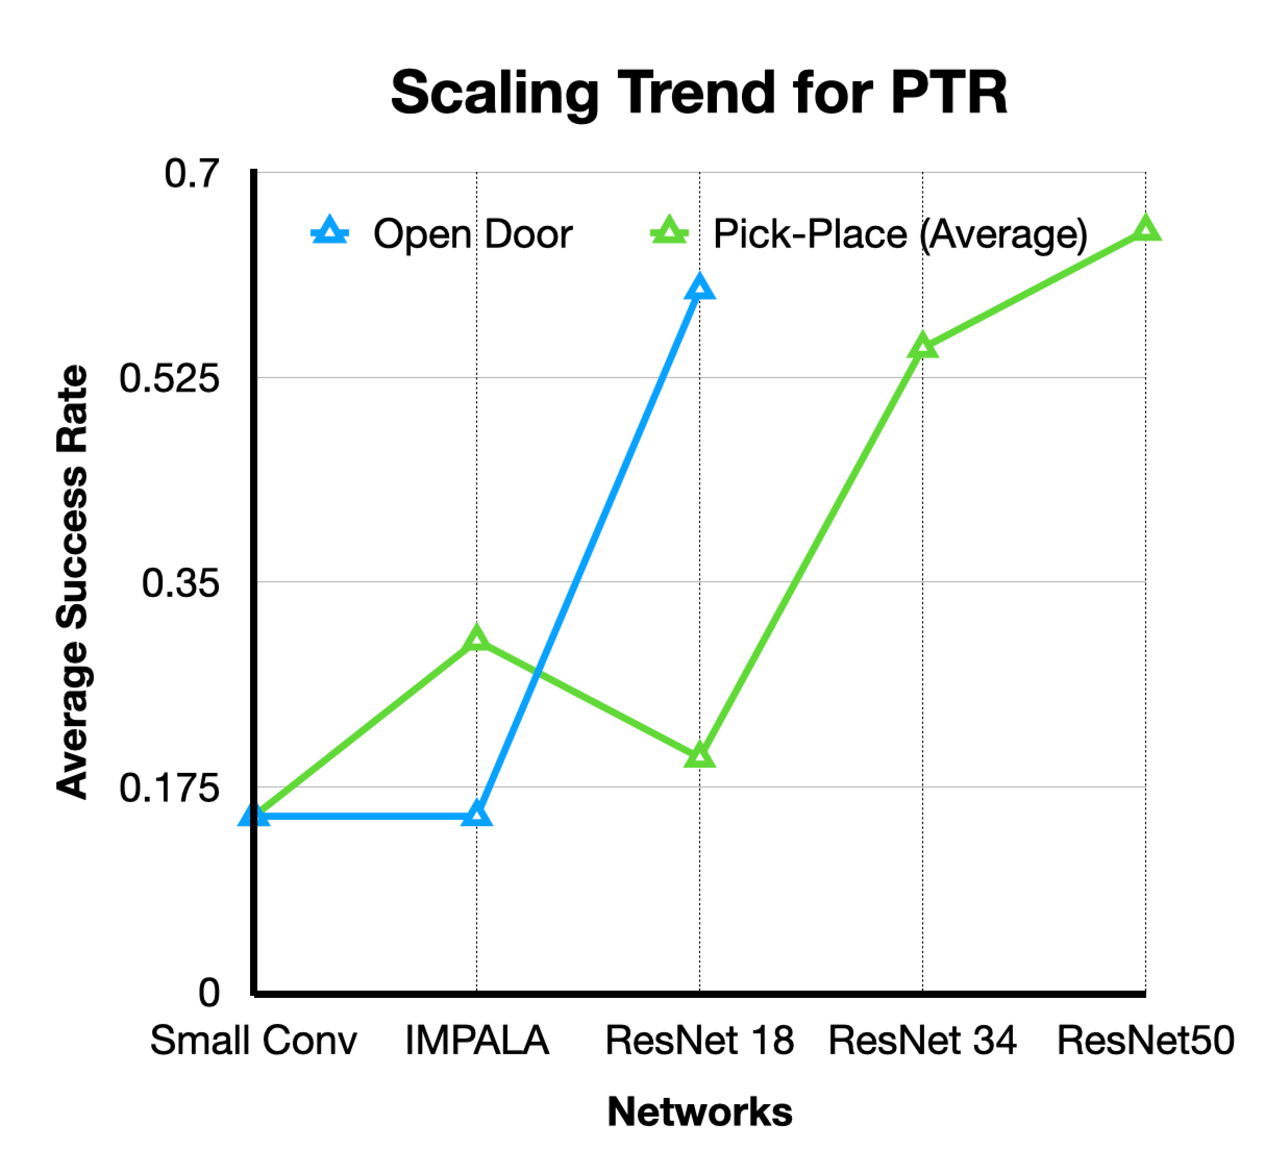
\includegraphics[width=0.6\linewidth]{chapters/ptr/scaling_ptr.pdf}
\vspace{-0.24cm}
\caption{\footnotesize{\label{fig:scaling_ptr} \textbf{Scaling trends for \ptrmethodname} on the open door task, and average over two pick and place tasks from Scenario 3. Note that with our design decisions, PTR is able to effectively benefit from high capacity networks.}}
\vspace{-0.6cm}
\end{figure}
To understand the importance of designing techniques that enable us to use high-capacity models for offline RL, we examine the efficacy of PTR with different neural network architectures on the open door task from Scenario 2, and the put cucumber in pot and take croissant out of metallic bowl tasks from Scenario 3. We compare to standard three-layer convolutional network architectures used by prior work for Deepmind control suite tasks (see for example, \citet{kostrikov2020image}), an IMPALA~\citep{espeholt2018impala} ResNet that consists of 15 convolutional layers spread across a stack of 3 residual blocks, and the ResNet 18, 34, and 50 architectures with our proposed design decisions. Observe in Figure~\ref{fig:scaling_ptr} that the performance of smaller networks (Small, IMPALA) is significantly worse than the ResNet in the door opening task. For the pick-and-place tasks that contain a much larger dataset, Small, IMPALA and ResNet18 all perform much worse than ResNet 34 and ResNet 50. In Appendix~\ref{app:design} we show that ResNet 34 models perform much worse if our prescribed design decisions are not used. 


\vspace{0.1cm}
\subsection{Autonomous Online Fine-Tuning}
\label{sec:experiments_online}
\vspace{0.1cm}





\begin{table}
% \small{
\centering
% \vspace{0.1cm}
\resizebox{0.8\linewidth}{!}{\begin{tabular}{c|c|c}
\toprule
& \textbf{SACfD} &  \textbf{\ptrmethodname (offline $\rightarrow$ online)}  \\ \midrule
All positions & 0\% $\rightarrow$ 0\%   &  \textbf{53\%  $\rightarrow$ 73\%} \\
Novel OOD positions & 0\% $\rightarrow$ 0\%  & \textbf{13\%  $\rightarrow$  60\%} \\
\bottomrule
\end{tabular}}
% \vspace{-0.3cm}
\caption{\footnotesize{\textbf{Performance before and after online fine-tuning.} The success rate of the \ptrmethodname pre-trained policy is improved significantly from online fine-tuning, especially on novel out-of-distribution (OOD) initial positions that must be learned entirely from autonomous interaction in the real world. The results are reported as the average of 3 trials from each initial position.}}
\vspace{-0.3cm}
\label{tab:online-finetune}
\end{table}

So far, we've evaluated \ptrmethodname with offline fine-tuning to new tasks. However, by pre-training representations with offline RL, we can also enable autonomous improvement through online RL fine-tuning. In this section, we will demonstrate this benefit by showing that an offline initialization learned by PTR pre-training can be effectively fine-tuned autonomously with online rollouts. This procedure provides a way forward to build self-improving robotic RL systems that bring the best of diverse robotic datasets and learning via online interaction.

\textbf{Task.} For this experiment, we consider the ``open door'' task from Scenario 2. Our goal is to improve the success rate of the learned policy obtained after PTR pre-training and offline fine-tuning using autonomous online rollouts from ten initial positions. These ten initial positions consist of five positions obtained by randomly sampling from the target demonstrations used for offline fine-tuning, and five more challenging \textbf{out-of-distribution initial positions}, that were never seen before.


\begin{figure}[t]
% \vspace{-0.7cm}
\centering
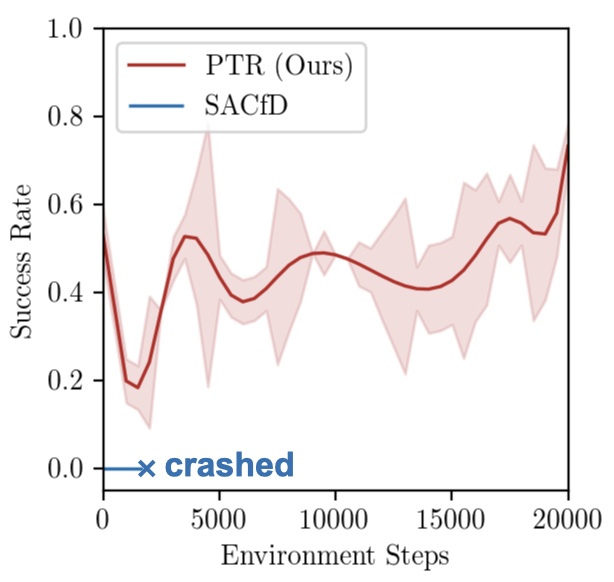
\includegraphics[width=0.6\linewidth]{chapters/ptr/online-open-door.jpeg}
\vspace{-0.24cm}
\caption{\footnotesize{\label{fig:online_door} \textbf{Online fine-tuning for \ptrmethodname} on the open door task. \ptrmethodname improves the success rate of the pre-trained policy from 53\% to 73\% (from 13\% to 60\% for the harder positions), while SACfD crashes due to unsafe behavior during exploration. We ran \ptrmethodname online fine-tuning for 2 seeds in the real world.}}
\vspace{-0.6cm}
\end{figure}

\textbf{Reward functions.} To run RL, we need a mechanism to annotate every online rollout with a reward signal. Following prior works~\citep{singh2019, kalashnikov2021mt}, we trained a neural-network binary classifier to detect a given visual observation as a success (+1 reward) or failure (0 reward) and use it to annotate rollouts executed during online interaction. 

\textbf{Reset policy.} To run online fine-tuning autonomously without any human intervention in the real world, we also need a ``reset policy'' that closes the door after a successful online rollout. To this end, we also pre-trained a close-door policy separately, which is used only for resetting the door. Note that online fine-tuning only fine-tunes the open-door policy, while the reset policy is kept fixed throughout.


\textbf{Online training setup.} Equipped with the reset policy and the reward classifier, we are able to run online fine-tuning in the real world. Starting from the pre-trained policy obtained via PTR, our method alternates between collecting a new trajectory and taking gradient steps. The update-to-data ratio~\citep{2021arXiv210105982C} is set to 10, which means that we  make 10 gradient updates for every environment step. More details about our implementation and evaluations can be found in Appendix~\ref{app:online_finetuning}.


\begin{figure}
\vspace{-0.4cm}
\centering
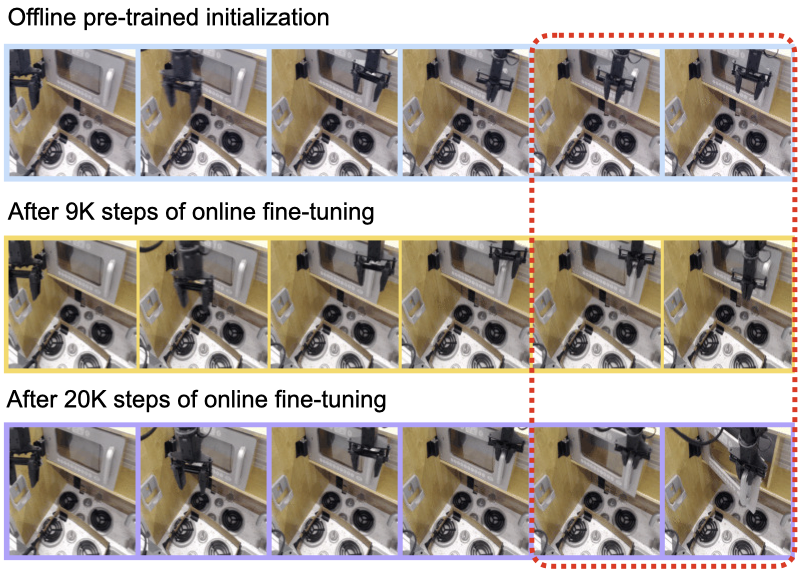
\includegraphics[width=0.85\linewidth]{chapters/ptr/online_improvement.png}
\vspace{-0.24cm}
\caption{\footnotesize{\label{fig:online-improvement} \textbf{Evolution of learned behaviors during autonomous online fine-tuning of PTR starting from one of the hard initial positions.} The blue box illustrates that the offline initialization fails to grasp the handle. After 9K steps of online interaction, it successfully grasps the handle but fails to open the door. After 20K steps, it learns to successfully open the door.}}
\vspace{-0.4cm}
\end{figure}

\textbf{Results.} We compare our method with a prior method that trains SAC~\citep{haarnoja2018soft} from scratch using both online data and offline demonstrations (denoted by ``SACfD''). This approach is an improved version of DDPGfD~\citep{vecerik2017leveraging} which uses a stronger off-policy RL algorithm (SAC). We present the learning curve during the online fine-tuning in Figure~\ref{fig:online_door}, and the success rates before and after fine-tuning in Table~\ref{tab:online-finetune}. As shown in Figure~\ref{fig:online_door}, it was difficult to run SACfD over a long time on the robot, as the system crashes due to unsafe actions during exploration (pictures shown in Appendix~\ref{app:online_finetuning}). In contrast, the pre-trained PTR policy is able to perform online exploration in a stable manner, and improve the success rate of the pre-trained policy within 20K steps of online interaction. Specifically, this boost in performance stems from learning to solve the task from \textbf{3/5} of the more challenging, out-of-distribution initial positions,
that were never seen before in the prior data, as shown in Figure~\ref{fig:online-improvement}. Overall, our results show the efficacy of PTR as a general-purpose pre-training paradigm for robotic RL. 

\section{Related Work}
\label{sec:related}

% A number of prior works have proposed algorithms for offline RL~\citep{fujimoto2018off,kumar2019stabilizing,kumar2020conservative,kostrikov2021offline,kostrikov2021iql,wu2019behavior,jaques2019way,fujimoto2021minimalist,siegel2020keep}. In particular, many prior works study offline RL with multi-task data and devise techniques that perform parameter sharing\citep{wilson2007multi, parisotto2015actor, teh2017distral, espeholt2018impala, hessel2019multi}, or perform data sharing or relabeling~\citep{yu2021conservative,andrychowicz2017hindsight,yu2022leverage,kalashnikov2021mt,xie2021lifelong}. In this paper, our goal is not to develop new offline RL algorithms, but to show that these offline RL algorithms can be an effective tool to pre-train from prior data and then fine-tune on new tasks. We show that a few simple but important design decisions are essential for making offline RL pre-training scalable, and provide detailed experiments on fine-tuning these pre-trained models to new tasks.

While a number of prior works have developed offline RL algorithms that can be applied to robotic conttrol as we discussed in previous chapters of this dissertation, in this chapter, we do not propose a new algorithm. Instead, our goal is to develop design decisions that can make existing offline RL methods an effective tool to pre-train from prior data and then fine-tune on new tasks. While these design decisions are simple, they are crucial, and substantially improve performance.

Going beyond methods that only perform fine-tuning from a learned initialization with online interaction~\citep{nair2020accelerating,kostrikov2021iql,lee2022offline} as we studied in the previous section of this dissertation, we consider two independent fine-tuning settings in this chapter: (1) the setting where we do not use any online interaction and fine-tune the pre-trained policy entirely offline, (2) the setting where a limited amount of online interaction is allowed to autonomously acquire the skills to solve the task from a challenging initial condition. This resembles the problem setting considered by offline meta-RL methods~\citep{li2019multi, dorfman2020offline, mitchell2021offline, pong2021offline,lin2022model}. However, our approach is simpler as we fine-tune the very same offline RL algorithm that we use for pre-training, without any distinct meta updates. In our experiments, we observe that our method, PTR, outperforms the meta-RL method of \citet{mitchell2021offline}. 

Some other prior approaches that attempt to leverage large, diverse datasets via representation learning~\citep{mandlekar2020iris,yang2021representation,yang2021trail,nair2022r3m,he2111masked,xiao2022masked,ma2022vip},
as well as other methods for learning from human demonstrations, such as behavioral cloning methods with expressive policy architectures~\citep{shafiullah2022behavior}.
We compare to some of these methods~\citep{xiao2022masked,nair2022r3m} in our experiments and find that PTR outperforms these methods. We also perform an empirical study to identify the design decisions behind the improved performance of RL-based PTR on demonstration data compared to BC, and find that the gains largely come from the ability of the value function in identifying the most ``critical'' decisions in a trajectory. 
% While some prior works~\citep{mandlekar2021what} shows results that suggest that offline RL underperforms imitation learning when provided with human demonstration data, our results show that offline RL can perform better than BC even with demonstrations, supporting the analysis in \citet{kumar2022should}.

The most closely related to our approach are prior methods that run model-free offline RL on diverse real-world data and then fine-tune on new tasks~\citep{singh2020cog,kalashnikov2021mt,julian2020never,chebotar2021actionable,lee2022spend}.
These prior methods typically only consider the setting of \emph{online} fine-tuning, whereas in our experiments, we demonstrate the efficacy of PTR for offline fine-tuning (where we must acquire a good policy for the downstream task using 10-15 demonstrations) \emph{as well as} online fine-tuning considered in these prior works, where we must acquire a new task entirely via autonomous interaction in the real world. 


\section{Discussion and Limitations}
\label{sec:conclusion}
We presented a system that uses diverse prior data for general-purpose offline RL pre-training, followed by fine-tuning to downstream tasks. The prior data, sourced from a publicly available dataset, consists of over a hundred tasks across ten scenes and our policies can be fine-tuned with as few as 10 demonstrations. We show that this approach outperforms prior pre-training and fine-tuning methods based on imitation learning. One of the most exciting directions for future work is to further scale up this pre-training to provide a single policy initialization, that can be utilized as a starting point, similar to GPT3~\citep{brown2020language}. 
An exciting future direction is to scale PTR up to more complex settings, including to novel robots. {Since joint training with offline RL was worse than pre-training and then fine-tuning with PTR, another exciting direction for future work is to understand the pros and cons of joint training and fine-tuning in the context of robot learning.}

\end{document}
